% ####################################################################
% Basic configuration of Beamera class and Jagiellonian theme
% ####################################################################
\RequirePackage[l2tabu, orthodox]{nag}



\ifx\PresentationStyle\notset
  \def\PresentationStyle{dark}
\fi



% Options: t - align frame text to the top.
\documentclass[10pt,t]{beamer}
\mode<presentation>
\usetheme[style=\PresentationStyle]{jagiellonian}




% ------------------------------------------------------------------------------------
% Procesing configuration files of Jagiellonian theme located
% in the directory "preambule"
% ------------------------------------------------------------------------------------
% Configuration for polish language
% Need description
\usepackage[polish]{babel}
% Need description
\usepackage[MeX]{polski}



% ------------------------------
% Better support of polish chars in technical parts of PDF
% ------------------------------
\hypersetup{pdfencoding=auto,psdextra}

% Package "textpos" give as enviroment "textblock" which is very usefull in
% arranging text on slides.

% This is standard configuration of "textpos"
\usepackage[overlay,absolute]{textpos}

% If you need to see bounds of "textblock's" comment line above and uncomment
% one below.

% Caution! When showboxes option is on significant ammunt of space is add
% to the top of textblock and as such, everyting put in them gone down.
% We need to check how to remove this bug.

% \usepackage[showboxes,overlay,absolute]{textpos}



% Setting scale length for package "textpos"
\setlength{\TPHorizModule}{10mm}
\setlength{\TPVertModule}{\TPHorizModule}


% ---------------------------------------
% Packages written for lectures "Geometria 3D dla twórców gier wideo"
% ---------------------------------------
% \usepackage{./Geometry3DPackages/Geometry3D}
% \usepackage{./Geometry3DPackages/Geometry3DIndices}
% \usepackage{./Geometry3DPackages/Geometry3DTikZStyle}
% \usepackage{./ProgramowanieSymulacjiFizykiPaczki/ProgramowanieSymulacjiFizykiTikZStyle}
% \usepackage{./Geometry3DPackages/mathcommands}


% ---------------------------------------
% Importing TikZ's libraries
% ---------------------------------------
\usetikzlibrary{arrows.meta}
\usetikzlibrary{positioning}





% % Configuration package "bm" that need for making bold symbols
\newcommand{\bmmax}{0}
\newcommand{\hmmax}{0}
\usepackage{bm}




% ---------------------------------------
% Packages for scientific texts
% ---------------------------------------
% \let\lll\undefined  % Sometimes you must use this line to allow
% "amsmath" package to works with packages with packages for polish
% languge imported
% /preambul/LanguageSettings/JagiellonianPolishLanguageSettings.tex.
% This comments (probably) removes polish letter Ł.
\usepackage{amsmath}  % Packages from American Mathematical Society (AMS)
\usepackage{amssymb}
\usepackage{amscd}
\usepackage{amsthm}
\usepackage{siunitx}  % Package for typsetting SI units.
\usepackage{upgreek}  % Better looking greek letters.
% Example of using upgreek: pi = \uppi


\usepackage{calrsfs}  % Zmienia czcionkę kaligraficzną w \mathcal
% na ładniejszą. Może w innych miejscach robi to samo, ale o tym nic
% nie wiem.







% !!!!!!!!!!!!!!!!!!!!!!!!!!!!!!
% !!!!!!!!!!!!!!!!!!!!!!!!!!!!!!
% EVIL STUFF
\if\JUlogotitle1
\edef\LogoJUPath{LogoJU_\JUlogoLang/LogoJU_\JUlogoShape_\JUlogoColor.pdf}
\titlegraphic{\hfill\includegraphics[scale=0.22]
{./JagiellonianPictures/\LogoJUPath}}
\fi

% ---------------------------------------
% Commands for handling colors
% ---------------------------------------


% Command for setting normal text color for some text in math modestyle
% Text color depend on used style of Jagiellonian

% Beamer version of command
\newcommand{\TextWithNormalTextColor}[1]{%
  {\color{jNormalTextFGColor}
    \setbeamercolor{math text}{fg=jNormalTextFGColor} {#1}}
}

% Article and similar classes version of command
% \newcommand{\TextWithNormalTextColor}[1]{%
%   {\color{jNormalTextsFGColor} {#1}}
% }



% Beamer version of command
\newcommand{\NormalTextInMathMode}[1]{%
  {\color{jNormalTextFGColor}
    \setbeamercolor{math text}{fg=jNormalTextFGColor} \text{#1}}
}


% Article and similar classes version of command
% \newcommand{\NormalTextInMathMode}[1]{%
%   {\color{jNormalTextsFGColor} \text{#1}}
% }




% Command that sets color of some mathematical text to the same color
% that has normal text in header (?)

% Beamer version of the command
\newcommand{\MathTextFrametitleFGColor}[1]{%
  {\color{jFrametitleFGColor}
    \setbeamercolor{math text}{fg=jFrametitleFGColor} #1}
}

% Article and similar classes version of the command
% \newcommand{\MathTextWhiteColor}[1]{{\color{jFrametitleFGColor} #1}}





% Command for setting color of alert text for some text in math modestyle

% Beamer version of the command
\newcommand{\MathTextAlertColor}[1]{%
  {\color{jOrange} \setbeamercolor{math text}{fg=jOrange} #1}
}

% Article and similar classes version of the command
% \newcommand{\MathTextAlertColor}[1]{{\color{jOrange} #1}}





% Command that allow you to sets chosen color as the color of some text into
% math mode. Due to some nuances in the way that Beamer handle colors
% it not work in all cases. We hope that in the future we will improve it.

% Beamer version of the command
\newcommand{\SetMathTextColor}[2]{%
  {\color{#1} \setbeamercolor{math text}{fg=#1} #2}
}


% Article and similar classes version of the command
% \newcommand{\SetMathTextColor}[2]{{\color{#1} #2}}










% ---------------------------------------
% Commands for few special slides
% ---------------------------------------
\newcommand{\EndingSlide}[1]{%
  \begin{frame}[standout]

    \begingroup

    \color{jFrametitleFGColor}

    #1

    \endgroup

  \end{frame}
}










% ---------------------------------------
% Commands for setting background pictures for some slides
% ---------------------------------------
\newcommand{\TitleBackgroundPicture}
{./JagiellonianPictures/Backgrounds/LajkonikDark.png}
\newcommand{\SectionBackgroundPicture}
{./JagiellonianPictures/Backgrounds/LajkonikLight.png}



\newcommand{\TitleSlideWithPicture}{%
  \begingroup

  \usebackgroundtemplate{%
    \includegraphics[height=\paperheight]{\TitleBackgroundPicture}}

  \maketitle

  \endgroup
}





\newcommand{\SectionSlideWithPicture}[1]{%
  \begingroup

  \usebackgroundtemplate{%
    \includegraphics[height=\paperheight]{\SectionBackgroundPicture}}

  \setbeamercolor{titlelike}{fg=normal text.fg}

  \section{#1}

  \endgroup
}










% ---------------------------------------
% Commands for lectures "Geometria 3D dla twórców gier wideo"
% Polish version
% ---------------------------------------
% Komendy teraz wykomentowane były potrzebne, gdy loga były na niebieskim
% tle, nie na białym. A są na białym bo tego chcieli w biurze projektu.
% \newcommand{\FundingLogoWhitePicturePL}
% {./PresentationPictures/CommonPictures/logotypFundusze_biale_bez_tla2.pdf}
\newcommand{\FundingLogoColorPicturePL}
{./PresentationPictures/CommonPictures/European_Funds_color_PL.pdf}
% \newcommand{\EULogoWhitePicturePL}
% {./PresentationPictures/CommonPictures/logotypUE_biale_bez_tla2.pdf}
\newcommand{\EUSocialFundLogoColorPicturePL}
{./PresentationPictures/CommonPictures/EU_Social_Fund_color_PL.pdf}
% \newcommand{\ZintegrUJLogoWhitePicturePL}
% {./PresentationPictures/CommonPictures/zintegruj-logo-white.pdf}
\newcommand{\ZintegrUJLogoColorPicturePL}
{./PresentationPictures/CommonPictures/ZintegrUJ_color.pdf}
\newcommand{\JULogoColorPicturePL}
{./JagiellonianPictures/LogoJU_PL/LogoJU_A_color.pdf}





\newcommand{\GeometryThreeDSpecialBeginningSlidePL}{%
  \begin{frame}[standout]

    \begin{textblock}{11}(1,0.7)

      \begin{flushleft}

        \mdseries

        \footnotesize

        \color{jFrametitleFGColor}

        Materiał powstał w ramach projektu współfinansowanego ze środków
        Unii Europejskiej w ramach Europejskiego Funduszu Społecznego
        POWR.03.05.00-00-Z309/17-00.

      \end{flushleft}

    \end{textblock}





    \begin{textblock}{10}(0,2.2)

      \tikz \fill[color=jBackgroundStyleLight] (0,0) rectangle (12.8,-1.5);

    \end{textblock}


    \begin{textblock}{3.2}(1,2.45)

      \includegraphics[scale=0.3]{\FundingLogoColorPicturePL}

    \end{textblock}


    \begin{textblock}{2.5}(3.7,2.5)

      \includegraphics[scale=0.2]{\JULogoColorPicturePL}

    \end{textblock}


    \begin{textblock}{2.5}(6,2.4)

      \includegraphics[scale=0.1]{\ZintegrUJLogoColorPicturePL}

    \end{textblock}


    \begin{textblock}{4.2}(8.4,2.6)

      \includegraphics[scale=0.3]{\EUSocialFundLogoColorPicturePL}

    \end{textblock}

  \end{frame}
}



\newcommand{\GeometryThreeDTwoSpecialBeginningSlidesPL}{%
  \begin{frame}[standout]

    \begin{textblock}{11}(1,0.7)

      \begin{flushleft}

        \mdseries

        \footnotesize

        \color{jFrametitleFGColor}

        Materiał powstał w ramach projektu współfinansowanego ze środków
        Unii Europejskiej w ramach Europejskiego Funduszu Społecznego
        POWR.03.05.00-00-Z309/17-00.

      \end{flushleft}

    \end{textblock}





    \begin{textblock}{10}(0,2.2)

      \tikz \fill[color=jBackgroundStyleLight] (0,0) rectangle (12.8,-1.5);

    \end{textblock}


    \begin{textblock}{3.2}(1,2.45)

      \includegraphics[scale=0.3]{\FundingLogoColorPicturePL}

    \end{textblock}


    \begin{textblock}{2.5}(3.7,2.5)

      \includegraphics[scale=0.2]{\JULogoColorPicturePL}

    \end{textblock}


    \begin{textblock}{2.5}(6,2.4)

      \includegraphics[scale=0.1]{\ZintegrUJLogoColorPicturePL}

    \end{textblock}


    \begin{textblock}{4.2}(8.4,2.6)

      \includegraphics[scale=0.3]{\EUSocialFundLogoColorPicturePL}

    \end{textblock}

  \end{frame}





  \TitleSlideWithPicture
}



\newcommand{\GeometryThreeDSpecialEndingSlidePL}{%
  \begin{frame}[standout]

    \begin{textblock}{11}(1,0.7)

      \begin{flushleft}

        \mdseries

        \footnotesize

        \color{jFrametitleFGColor}

        Materiał powstał w ramach projektu współfinansowanego ze środków
        Unii Europejskiej w~ramach Europejskiego Funduszu Społecznego
        POWR.03.05.00-00-Z309/17-00.

      \end{flushleft}

    \end{textblock}





    \begin{textblock}{10}(0,2.2)

      \tikz \fill[color=jBackgroundStyleLight] (0,0) rectangle (12.8,-1.5);

    \end{textblock}


    \begin{textblock}{3.2}(1,2.45)

      \includegraphics[scale=0.3]{\FundingLogoColorPicturePL}

    \end{textblock}


    \begin{textblock}{2.5}(3.7,2.5)

      \includegraphics[scale=0.2]{\JULogoColorPicturePL}

    \end{textblock}


    \begin{textblock}{2.5}(6,2.4)

      \includegraphics[scale=0.1]{\ZintegrUJLogoColorPicturePL}

    \end{textblock}


    \begin{textblock}{4.2}(8.4,2.6)

      \includegraphics[scale=0.3]{\EUSocialFundLogoColorPicturePL}

    \end{textblock}





    \begin{textblock}{11}(1,4)

      \begin{flushleft}

        \mdseries

        \footnotesize

        \RaggedRight

        \color{jFrametitleFGColor}

        Treść niniejszego wykładu jest udostępniona na~licencji
        Creative Commons (\textsc{cc}), z~uzna\-niem autorstwa
        (\textsc{by}) oraz udostępnianiem na tych samych warunkach
        (\textsc{sa}). Rysunki i~wy\-kresy zawarte w~wykładzie są
        autorstwa dr.~hab.~Pawła Węgrzyna et~al. i~są dostępne
        na tej samej licencji, o~ile nie wskazano inaczej.
        W~prezentacji wykorzystano temat Beamera Jagiellonian,
        oparty na~temacie Metropolis Matthiasa Vogelgesanga,
        dostępnym na licencji \LaTeX{} Project Public License~1.3c
        pod adresem: \colorhref{https://github.com/matze/mtheme}
        {https://github.com/matze/mtheme}.

        Projekt typograficzny: Iwona Grabska-Gradzińska \\
        Skład: Kamil Ziemian;
        Korekta: Wojciech Palacz \\
        Modele: Dariusz Frymus, Kamil Nowakowski \\
        Rysunki i~wykresy: Kamil Ziemian, Paweł Węgrzyn, Wojciech Palacz

      \end{flushleft}

    \end{textblock}

  \end{frame}
}



\newcommand{\GeometryThreeDTwoSpecialEndingSlidesPL}[1]{%
  \begin{frame}[standout]


    \begin{textblock}{11}(1,0.7)

      \begin{flushleft}

        \mdseries

        \footnotesize

        \color{jFrametitleFGColor}

        Materiał powstał w ramach projektu współfinansowanego ze środków
        Unii Europejskiej w~ramach Europejskiego Funduszu Społecznego
        POWR.03.05.00-00-Z309/17-00.

      \end{flushleft}

    \end{textblock}





    \begin{textblock}{10}(0,2.2)

      \tikz \fill[color=jBackgroundStyleLight] (0,0) rectangle (12.8,-1.5);

    \end{textblock}


    \begin{textblock}{3.2}(1,2.45)

      \includegraphics[scale=0.3]{\FundingLogoColorPicturePL}

    \end{textblock}


    \begin{textblock}{2.5}(3.7,2.5)

      \includegraphics[scale=0.2]{\JULogoColorPicturePL}

    \end{textblock}


    \begin{textblock}{2.5}(6,2.4)

      \includegraphics[scale=0.1]{\ZintegrUJLogoColorPicturePL}

    \end{textblock}


    \begin{textblock}{4.2}(8.4,2.6)

      \includegraphics[scale=0.3]{\EUSocialFundLogoColorPicturePL}

    \end{textblock}





    \begin{textblock}{11}(1,4)

      \begin{flushleft}

        \mdseries

        \footnotesize

        \RaggedRight

        \color{jFrametitleFGColor}

        Treść niniejszego wykładu jest udostępniona na~licencji
        Creative Commons (\textsc{cc}), z~uzna\-niem autorstwa
        (\textsc{by}) oraz udostępnianiem na tych samych warunkach
        (\textsc{sa}). Rysunki i~wy\-kresy zawarte w~wykładzie są
        autorstwa dr.~hab.~Pawła Węgrzyna et~al. i~są dostępne
        na tej samej licencji, o~ile nie wskazano inaczej.
        W~prezentacji wykorzystano temat Beamera Jagiellonian,
        oparty na~temacie Metropolis Matthiasa Vogelgesanga,
        dostępnym na licencji \LaTeX{} Project Public License~1.3c
        pod adresem: \colorhref{https://github.com/matze/mtheme}
        {https://github.com/matze/mtheme}.

        Projekt typograficzny: Iwona Grabska-Gradzińska \\
        Skład: Kamil Ziemian;
        Korekta: Wojciech Palacz \\
        Modele: Dariusz Frymus, Kamil Nowakowski \\
        Rysunki i~wykresy: Kamil Ziemian, Paweł Węgrzyn, Wojciech Palacz

      \end{flushleft}

    \end{textblock}

  \end{frame}





  \begin{frame}[standout]

    \begingroup

    \color{jFrametitleFGColor}

    #1

    \endgroup

  \end{frame}
}



\newcommand{\GeometryThreeDSpecialEndingSlideVideoPL}{%
  \begin{frame}[standout]

    \begin{textblock}{11}(1,0.7)

      \begin{flushleft}

        \mdseries

        \footnotesize

        \color{jFrametitleFGColor}

        Materiał powstał w ramach projektu współfinansowanego ze środków
        Unii Europejskiej w~ramach Europejskiego Funduszu Społecznego
        POWR.03.05.00-00-Z309/17-00.

      \end{flushleft}

    \end{textblock}





    \begin{textblock}{10}(0,2.2)

      \tikz \fill[color=jBackgroundStyleLight] (0,0) rectangle (12.8,-1.5);

    \end{textblock}


    \begin{textblock}{3.2}(1,2.45)

      \includegraphics[scale=0.3]{\FundingLogoColorPicturePL}

    \end{textblock}


    \begin{textblock}{2.5}(3.7,2.5)

      \includegraphics[scale=0.2]{\JULogoColorPicturePL}

    \end{textblock}


    \begin{textblock}{2.5}(6,2.4)

      \includegraphics[scale=0.1]{\ZintegrUJLogoColorPicturePL}

    \end{textblock}


    \begin{textblock}{4.2}(8.4,2.6)

      \includegraphics[scale=0.3]{\EUSocialFundLogoColorPicturePL}

    \end{textblock}





    \begin{textblock}{11}(1,4)

      \begin{flushleft}

        \mdseries

        \footnotesize

        \RaggedRight

        \color{jFrametitleFGColor}

        Treść niniejszego wykładu jest udostępniona na~licencji
        Creative Commons (\textsc{cc}), z~uzna\-niem autorstwa
        (\textsc{by}) oraz udostępnianiem na tych samych warunkach
        (\textsc{sa}). Rysunki i~wy\-kresy zawarte w~wykładzie są
        autorstwa dr.~hab.~Pawła Węgrzyna et~al. i~są dostępne
        na tej samej licencji, o~ile nie wskazano inaczej.
        W~prezentacji wykorzystano temat Beamera Jagiellonian,
        oparty na~temacie Metropolis Matthiasa Vogelgesanga,
        dostępnym na licencji \LaTeX{} Project Public License~1.3c
        pod adresem: \colorhref{https://github.com/matze/mtheme}
        {https://github.com/matze/mtheme}.

        Projekt typograficzny: Iwona Grabska-Gradzińska;
        Skład: Kamil Ziemian \\
        Korekta: Wojciech Palacz;
        Modele: Dariusz Frymus, Kamil Nowakowski \\
        Rysunki i~wykresy: Kamil Ziemian, Paweł Węgrzyn, Wojciech Palacz \\
        Montaż: Agencja Filmowa Film \& Television Production~-- Zbigniew
        Masklak

      \end{flushleft}

    \end{textblock}

  \end{frame}
}





\newcommand{\GeometryThreeDTwoSpecialEndingSlidesVideoPL}[1]{%
  \begin{frame}[standout]

    \begin{textblock}{11}(1,0.7)

      \begin{flushleft}

        \mdseries

        \footnotesize

        \color{jFrametitleFGColor}

        Materiał powstał w ramach projektu współfinansowanego ze środków
        Unii Europejskiej w~ramach Europejskiego Funduszu Społecznego
        POWR.03.05.00-00-Z309/17-00.

      \end{flushleft}

    \end{textblock}





    \begin{textblock}{10}(0,2.2)

      \tikz \fill[color=jBackgroundStyleLight] (0,0) rectangle (12.8,-1.5);

    \end{textblock}


    \begin{textblock}{3.2}(1,2.45)

      \includegraphics[scale=0.3]{\FundingLogoColorPicturePL}

    \end{textblock}


    \begin{textblock}{2.5}(3.7,2.5)

      \includegraphics[scale=0.2]{\JULogoColorPicturePL}

    \end{textblock}


    \begin{textblock}{2.5}(6,2.4)

      \includegraphics[scale=0.1]{\ZintegrUJLogoColorPicturePL}

    \end{textblock}


    \begin{textblock}{4.2}(8.4,2.6)

      \includegraphics[scale=0.3]{\EUSocialFundLogoColorPicturePL}

    \end{textblock}





    \begin{textblock}{11}(1,4)

      \begin{flushleft}

        \mdseries

        \footnotesize

        \RaggedRight

        \color{jFrametitleFGColor}

        Treść niniejszego wykładu jest udostępniona na~licencji
        Creative Commons (\textsc{cc}), z~uzna\-niem autorstwa
        (\textsc{by}) oraz udostępnianiem na tych samych warunkach
        (\textsc{sa}). Rysunki i~wy\-kresy zawarte w~wykładzie są
        autorstwa dr.~hab.~Pawła Węgrzyna et~al. i~są dostępne
        na tej samej licencji, o~ile nie wskazano inaczej.
        W~prezentacji wykorzystano temat Beamera Jagiellonian,
        oparty na~temacie Metropolis Matthiasa Vogelgesanga,
        dostępnym na licencji \LaTeX{} Project Public License~1.3c
        pod adresem: \colorhref{https://github.com/matze/mtheme}
        {https://github.com/matze/mtheme}.

        Projekt typograficzny: Iwona Grabska-Gradzińska;
        Skład: Kamil Ziemian \\
        Korekta: Wojciech Palacz;
        Modele: Dariusz Frymus, Kamil Nowakowski \\
        Rysunki i~wykresy: Kamil Ziemian, Paweł Węgrzyn, Wojciech Palacz \\
        Montaż: Agencja Filmowa Film \& Television Production~-- Zbigniew
        Masklak

      \end{flushleft}

    \end{textblock}

  \end{frame}





  \begin{frame}[standout]


    \begingroup

    \color{jFrametitleFGColor}

    #1

    \endgroup

  \end{frame}
}










% ---------------------------------------
% Commands for lectures "Geometria 3D dla twórców gier wideo"
% English version
% ---------------------------------------
% \newcommand{\FundingLogoWhitePictureEN}
% {./PresentationPictures/CommonPictures/logotypFundusze_biale_bez_tla2.pdf}
\newcommand{\FundingLogoColorPictureEN}
{./PresentationPictures/CommonPictures/European_Funds_color_EN.pdf}
% \newcommand{\EULogoWhitePictureEN}
% {./PresentationPictures/CommonPictures/logotypUE_biale_bez_tla2.pdf}
\newcommand{\EUSocialFundLogoColorPictureEN}
{./PresentationPictures/CommonPictures/EU_Social_Fund_color_EN.pdf}
% \newcommand{\ZintegrUJLogoWhitePictureEN}
% {./PresentationPictures/CommonPictures/zintegruj-logo-white.pdf}
\newcommand{\ZintegrUJLogoColorPictureEN}
{./PresentationPictures/CommonPictures/ZintegrUJ_color.pdf}
\newcommand{\JULogoColorPictureEN}
{./JagiellonianPictures/LogoJU_EN/LogoJU_A_color.pdf}



\newcommand{\GeometryThreeDSpecialBeginningSlideEN}{%
  \begin{frame}[standout]

    \begin{textblock}{11}(1,0.7)

      \begin{flushleft}

        \mdseries

        \footnotesize

        \color{jFrametitleFGColor}

        This content was created as part of a project co-financed by the
        European Union within the framework of the European Social Fund
        POWR.03.05.00-00-Z309/17-00.

      \end{flushleft}

    \end{textblock}





    \begin{textblock}{10}(0,2.2)

      \tikz \fill[color=jBackgroundStyleLight] (0,0) rectangle (12.8,-1.5);

    \end{textblock}


    \begin{textblock}{3.2}(0.7,2.45)

      \includegraphics[scale=0.3]{\FundingLogoColorPictureEN}

    \end{textblock}


    \begin{textblock}{2.5}(4.15,2.5)

      \includegraphics[scale=0.2]{\JULogoColorPictureEN}

    \end{textblock}


    \begin{textblock}{2.5}(6.35,2.4)

      \includegraphics[scale=0.1]{\ZintegrUJLogoColorPictureEN}

    \end{textblock}


    \begin{textblock}{4.2}(8.4,2.6)

      \includegraphics[scale=0.3]{\EUSocialFundLogoColorPictureEN}

    \end{textblock}

  \end{frame}
}



\newcommand{\GeometryThreeDTwoSpecialBeginningSlidesEN}{%
  \begin{frame}[standout]

    \begin{textblock}{11}(1,0.7)

      \begin{flushleft}

        \mdseries

        \footnotesize

        \color{jFrametitleFGColor}

        This content was created as part of a project co-financed by the
        European Union within the framework of the European Social Fund
        POWR.03.05.00-00-Z309/17-00.

      \end{flushleft}

    \end{textblock}





    \begin{textblock}{10}(0,2.2)

      \tikz \fill[color=jBackgroundStyleLight] (0,0) rectangle (12.8,-1.5);

    \end{textblock}


    \begin{textblock}{3.2}(0.7,2.45)

      \includegraphics[scale=0.3]{\FundingLogoColorPictureEN}

    \end{textblock}


    \begin{textblock}{2.5}(4.15,2.5)

      \includegraphics[scale=0.2]{\JULogoColorPictureEN}

    \end{textblock}


    \begin{textblock}{2.5}(6.35,2.4)

      \includegraphics[scale=0.1]{\ZintegrUJLogoColorPictureEN}

    \end{textblock}


    \begin{textblock}{4.2}(8.4,2.6)

      \includegraphics[scale=0.3]{\EUSocialFundLogoColorPictureEN}

    \end{textblock}

  \end{frame}





  \TitleSlideWithPicture
}



\newcommand{\GeometryThreeDSpecialEndingSlideEN}{%
  \begin{frame}[standout]

    \begin{textblock}{11}(1,0.7)

      \begin{flushleft}

        \mdseries

        \footnotesize

        \color{jFrametitleFGColor}

        This content was created as part of a project co-financed by the
        European Union within the framework of the European Social Fund
        POWR.03.05.00-00-Z309/17-00.

      \end{flushleft}

    \end{textblock}





    \begin{textblock}{10}(0,2.2)

      \tikz \fill[color=jBackgroundStyleLight] (0,0) rectangle (12.8,-1.5);

    \end{textblock}


    \begin{textblock}{3.2}(0.7,2.45)

      \includegraphics[scale=0.3]{\FundingLogoColorPictureEN}

    \end{textblock}


    \begin{textblock}{2.5}(4.15,2.5)

      \includegraphics[scale=0.2]{\JULogoColorPictureEN}

    \end{textblock}


    \begin{textblock}{2.5}(6.35,2.4)

      \includegraphics[scale=0.1]{\ZintegrUJLogoColorPictureEN}

    \end{textblock}


    \begin{textblock}{4.2}(8.4,2.6)

      \includegraphics[scale=0.3]{\EUSocialFundLogoColorPictureEN}

    \end{textblock}





    \begin{textblock}{11}(1,4)

      \begin{flushleft}

        \mdseries

        \footnotesize

        \RaggedRight

        \color{jFrametitleFGColor}

        The content of this lecture is made available under a~Creative
        Commons licence (\textsc{cc}), giving the author the credits
        (\textsc{by}) and putting an obligation to share on the same terms
        (\textsc{sa}). Figures and diagrams included in the lecture are
        authored by Paweł Węgrzyn et~al., and are available under the same
        license unless indicated otherwise.\\ The presentation uses the
        Beamer Jagiellonian theme based on Matthias Vogelgesang’s
        Metropolis theme, available under license \LaTeX{} Project
        Public License~1.3c at: \colorhref{https://github.com/matze/mtheme}
        {https://github.com/matze/mtheme}.

        Typographic design: Iwona Grabska-Gradzińska \\
        \LaTeX{} Typesetting: Kamil Ziemian \\
        Proofreading: Wojciech Palacz,
        Monika Stawicka \\
        3D Models: Dariusz Frymus, Kamil Nowakowski \\
        Figures and charts: Kamil Ziemian, Paweł Węgrzyn, Wojciech Palacz

      \end{flushleft}

    \end{textblock}

  \end{frame}
}



\newcommand{\GeometryThreeDTwoSpecialEndingSlidesEN}[1]{%
  \begin{frame}[standout]


    \begin{textblock}{11}(1,0.7)

      \begin{flushleft}

        \mdseries

        \footnotesize

        \color{jFrametitleFGColor}

        This content was created as part of a project co-financed by the
        European Union within the framework of the European Social Fund
        POWR.03.05.00-00-Z309/17-00.

      \end{flushleft}

    \end{textblock}





    \begin{textblock}{10}(0,2.2)

      \tikz \fill[color=jBackgroundStyleLight] (0,0) rectangle (12.8,-1.5);

    \end{textblock}


    \begin{textblock}{3.2}(0.7,2.45)

      \includegraphics[scale=0.3]{\FundingLogoColorPictureEN}

    \end{textblock}


    \begin{textblock}{2.5}(4.15,2.5)

      \includegraphics[scale=0.2]{\JULogoColorPictureEN}

    \end{textblock}


    \begin{textblock}{2.5}(6.35,2.4)

      \includegraphics[scale=0.1]{\ZintegrUJLogoColorPictureEN}

    \end{textblock}


    \begin{textblock}{4.2}(8.4,2.6)

      \includegraphics[scale=0.3]{\EUSocialFundLogoColorPictureEN}

    \end{textblock}





    \begin{textblock}{11}(1,4)

      \begin{flushleft}

        \mdseries

        \footnotesize

        \RaggedRight

        \color{jFrametitleFGColor}

        The content of this lecture is made available under a~Creative
        Commons licence (\textsc{cc}), giving the author the credits
        (\textsc{by}) and putting an obligation to share on the same terms
        (\textsc{sa}). Figures and diagrams included in the lecture are
        authored by Paweł Węgrzyn et~al., and are available under the same
        license unless indicated otherwise.\\ The presentation uses the
        Beamer Jagiellonian theme based on Matthias Vogelgesang’s
        Metropolis theme, available under license \LaTeX{} Project
        Public License~1.3c at: \colorhref{https://github.com/matze/mtheme}
        {https://github.com/matze/mtheme}.

        Typographic design: Iwona Grabska-Gradzińska \\
        \LaTeX{} Typesetting: Kamil Ziemian \\
        Proofreading: Wojciech Palacz,
        Monika Stawicka \\
        3D Models: Dariusz Frymus, Kamil Nowakowski \\
        Figures and charts: Kamil Ziemian, Paweł Węgrzyn, Wojciech Palacz

      \end{flushleft}

    \end{textblock}

  \end{frame}





  \begin{frame}[standout]

    \begingroup

    \color{jFrametitleFGColor}

    #1

    \endgroup

  \end{frame}
}



\newcommand{\GeometryThreeDSpecialEndingSlideVideoVerOneEN}{%
  \begin{frame}[standout]

    \begin{textblock}{11}(1,0.7)

      \begin{flushleft}

        \mdseries

        \footnotesize

        \color{jFrametitleFGColor}

        This content was created as part of a project co-financed by the
        European Union within the framework of the European Social Fund
        POWR.03.05.00-00-Z309/17-00.

      \end{flushleft}

    \end{textblock}





    \begin{textblock}{10}(0,2.2)

      \tikz \fill[color=jBackgroundStyleLight] (0,0) rectangle (12.8,-1.5);

    \end{textblock}


    \begin{textblock}{3.2}(0.7,2.45)

      \includegraphics[scale=0.3]{\FundingLogoColorPictureEN}

    \end{textblock}


    \begin{textblock}{2.5}(4.15,2.5)

      \includegraphics[scale=0.2]{\JULogoColorPictureEN}

    \end{textblock}


    \begin{textblock}{2.5}(6.35,2.4)

      \includegraphics[scale=0.1]{\ZintegrUJLogoColorPictureEN}

    \end{textblock}


    \begin{textblock}{4.2}(8.4,2.6)

      \includegraphics[scale=0.3]{\EUSocialFundLogoColorPictureEN}

    \end{textblock}





    \begin{textblock}{11}(1,4)

      \begin{flushleft}

        \mdseries

        \footnotesize

        \RaggedRight

        \color{jFrametitleFGColor}

        The content of this lecture is made available under a Creative
        Commons licence (\textsc{cc}), giving the author the credits
        (\textsc{by}) and putting an obligation to share on the same terms
        (\textsc{sa}). Figures and diagrams included in the lecture are
        authored by Paweł Węgrzyn et~al., and are available under the same
        license unless indicated otherwise.\\ The presentation uses the
        Beamer Jagiellonian theme based on Matthias Vogelgesang’s
        Metropolis theme, available under license \LaTeX{} Project
        Public License~1.3c at: \colorhref{https://github.com/matze/mtheme}
        {https://github.com/matze/mtheme}.

        Typographic design: Iwona Grabska-Gradzińska;
        \LaTeX{} Typesetting: Kamil Ziemian \\
        Proofreading: Wojciech Palacz,
        Monika Stawicka \\
        3D Models: Dariusz Frymus, Kamil Nowakowski \\
        Figures and charts: Kamil Ziemian, Paweł Węgrzyn, Wojciech
        Palacz \\
        Film editing: Agencja Filmowa Film \& Television Production~--
        Zbigniew Masklak

      \end{flushleft}

    \end{textblock}

  \end{frame}
}



\newcommand{\GeometryThreeDSpecialEndingSlideVideoVerTwoEN}{%
  \begin{frame}[standout]

    \begin{textblock}{11}(1,0.7)

      \begin{flushleft}

        \mdseries

        \footnotesize

        \color{jFrametitleFGColor}

        This content was created as part of a project co-financed by the
        European Union within the framework of the European Social Fund
        POWR.03.05.00-00-Z309/17-00.

      \end{flushleft}

    \end{textblock}





    \begin{textblock}{10}(0,2.2)

      \tikz \fill[color=jBackgroundStyleLight] (0,0) rectangle (12.8,-1.5);

    \end{textblock}


    \begin{textblock}{3.2}(0.7,2.45)

      \includegraphics[scale=0.3]{\FundingLogoColorPictureEN}

    \end{textblock}


    \begin{textblock}{2.5}(4.15,2.5)

      \includegraphics[scale=0.2]{\JULogoColorPictureEN}

    \end{textblock}


    \begin{textblock}{2.5}(6.35,2.4)

      \includegraphics[scale=0.1]{\ZintegrUJLogoColorPictureEN}

    \end{textblock}


    \begin{textblock}{4.2}(8.4,2.6)

      \includegraphics[scale=0.3]{\EUSocialFundLogoColorPictureEN}

    \end{textblock}





    \begin{textblock}{11}(1,4)

      \begin{flushleft}

        \mdseries

        \footnotesize

        \RaggedRight

        \color{jFrametitleFGColor}

        The content of this lecture is made available under a Creative
        Commons licence (\textsc{cc}), giving the author the credits
        (\textsc{by}) and putting an obligation to share on the same terms
        (\textsc{sa}). Figures and diagrams included in the lecture are
        authored by Paweł Węgrzyn et~al., and are available under the same
        license unless indicated otherwise.\\ The presentation uses the
        Beamer Jagiellonian theme based on Matthias Vogelgesang’s
        Metropolis theme, available under license \LaTeX{} Project
        Public License~1.3c at: \colorhref{https://github.com/matze/mtheme}
        {https://github.com/matze/mtheme}.

        Typographic design: Iwona Grabska-Gradzińska;
        \LaTeX{} Typesetting: Kamil Ziemian \\
        Proofreading: Wojciech Palacz,
        Monika Stawicka \\
        3D Models: Dariusz Frymus, Kamil Nowakowski \\
        Figures and charts: Kamil Ziemian, Paweł Węgrzyn, Wojciech
        Palacz \\
        Film editing: IMAVI -- Joanna Kozakiewicz, Krzysztof Magda, Nikodem
        Frodyma

      \end{flushleft}

    \end{textblock}

  \end{frame}
}



\newcommand{\GeometryThreeDSpecialEndingSlideVideoVerThreeEN}{%
  \begin{frame}[standout]

    \begin{textblock}{11}(1,0.7)

      \begin{flushleft}

        \mdseries

        \footnotesize

        \color{jFrametitleFGColor}

        This content was created as part of a project co-financed by the
        European Union within the framework of the European Social Fund
        POWR.03.05.00-00-Z309/17-00.

      \end{flushleft}

    \end{textblock}





    \begin{textblock}{10}(0,2.2)

      \tikz \fill[color=jBackgroundStyleLight] (0,0) rectangle (12.8,-1.5);

    \end{textblock}


    \begin{textblock}{3.2}(0.7,2.45)

      \includegraphics[scale=0.3]{\FundingLogoColorPictureEN}

    \end{textblock}


    \begin{textblock}{2.5}(4.15,2.5)

      \includegraphics[scale=0.2]{\JULogoColorPictureEN}

    \end{textblock}


    \begin{textblock}{2.5}(6.35,2.4)

      \includegraphics[scale=0.1]{\ZintegrUJLogoColorPictureEN}

    \end{textblock}


    \begin{textblock}{4.2}(8.4,2.6)

      \includegraphics[scale=0.3]{\EUSocialFundLogoColorPictureEN}

    \end{textblock}





    \begin{textblock}{11}(1,4)

      \begin{flushleft}

        \mdseries

        \footnotesize

        \RaggedRight

        \color{jFrametitleFGColor}

        The content of this lecture is made available under a Creative
        Commons licence (\textsc{cc}), giving the author the credits
        (\textsc{by}) and putting an obligation to share on the same terms
        (\textsc{sa}). Figures and diagrams included in the lecture are
        authored by Paweł Węgrzyn et~al., and are available under the same
        license unless indicated otherwise.\\ The presentation uses the
        Beamer Jagiellonian theme based on Matthias Vogelgesang’s
        Metropolis theme, available under license \LaTeX{} Project
        Public License~1.3c at: \colorhref{https://github.com/matze/mtheme}
        {https://github.com/matze/mtheme}.

        Typographic design: Iwona Grabska-Gradzińska;
        \LaTeX{} Typesetting: Kamil Ziemian \\
        Proofreading: Wojciech Palacz,
        Monika Stawicka \\
        3D Models: Dariusz Frymus, Kamil Nowakowski \\
        Figures and charts: Kamil Ziemian, Paweł Węgrzyn, Wojciech
        Palacz \\
        Film editing: Agencja Filmowa Film \& Television Production~--
        Zbigniew Masklak \\
        Film editing: IMAVI -- Joanna Kozakiewicz, Krzysztof Magda, Nikodem
        Frodyma

      \end{flushleft}

    \end{textblock}

  \end{frame}
}



\newcommand{\GeometryThreeDTwoSpecialEndingSlidesVideoVerOneEN}[1]{%
  \begin{frame}[standout]

    \begin{textblock}{11}(1,0.7)

      \begin{flushleft}

        \mdseries

        \footnotesize

        \color{jFrametitleFGColor}

        This content was created as part of a project co-financed by the
        European Union within the framework of the European Social Fund
        POWR.03.05.00-00-Z309/17-00.

      \end{flushleft}

    \end{textblock}





    \begin{textblock}{10}(0,2.2)

      \tikz \fill[color=jBackgroundStyleLight] (0,0) rectangle (12.8,-1.5);

    \end{textblock}


    \begin{textblock}{3.2}(0.7,2.45)

      \includegraphics[scale=0.3]{\FundingLogoColorPictureEN}

    \end{textblock}


    \begin{textblock}{2.5}(4.15,2.5)

      \includegraphics[scale=0.2]{\JULogoColorPictureEN}

    \end{textblock}


    \begin{textblock}{2.5}(6.35,2.4)

      \includegraphics[scale=0.1]{\ZintegrUJLogoColorPictureEN}

    \end{textblock}


    \begin{textblock}{4.2}(8.4,2.6)

      \includegraphics[scale=0.3]{\EUSocialFundLogoColorPictureEN}

    \end{textblock}





    \begin{textblock}{11}(1,4)

      \begin{flushleft}

        \mdseries

        \footnotesize

        \RaggedRight

        \color{jFrametitleFGColor}

        The content of this lecture is made available under a Creative
        Commons licence (\textsc{cc}), giving the author the credits
        (\textsc{by}) and putting an obligation to share on the same terms
        (\textsc{sa}). Figures and diagrams included in the lecture are
        authored by Paweł Węgrzyn et~al., and are available under the same
        license unless indicated otherwise.\\ The presentation uses the
        Beamer Jagiellonian theme based on Matthias Vogelgesang’s
        Metropolis theme, available under license \LaTeX{} Project
        Public License~1.3c at: \colorhref{https://github.com/matze/mtheme}
        {https://github.com/matze/mtheme}.

        Typographic design: Iwona Grabska-Gradzińska;
        \LaTeX{} Typesetting: Kamil Ziemian \\
        Proofreading: Wojciech Palacz,
        Monika Stawicka \\
        3D Models: Dariusz Frymus, Kamil Nowakowski \\
        Figures and charts: Kamil Ziemian, Paweł Węgrzyn,
        Wojciech Palacz \\
        Film editing: Agencja Filmowa Film \& Television Production~--
        Zbigniew Masklak

      \end{flushleft}

    \end{textblock}

  \end{frame}





  \begin{frame}[standout]


    \begingroup

    \color{jFrametitleFGColor}

    #1

    \endgroup

  \end{frame}
}



\newcommand{\GeometryThreeDTwoSpecialEndingSlidesVideoVerTwoEN}[1]{%
  \begin{frame}[standout]

    \begin{textblock}{11}(1,0.7)

      \begin{flushleft}

        \mdseries

        \footnotesize

        \color{jFrametitleFGColor}

        This content was created as part of a project co-financed by the
        European Union within the framework of the European Social Fund
        POWR.03.05.00-00-Z309/17-00.

      \end{flushleft}

    \end{textblock}





    \begin{textblock}{10}(0,2.2)

      \tikz \fill[color=jBackgroundStyleLight] (0,0) rectangle (12.8,-1.5);

    \end{textblock}


    \begin{textblock}{3.2}(0.7,2.45)

      \includegraphics[scale=0.3]{\FundingLogoColorPictureEN}

    \end{textblock}


    \begin{textblock}{2.5}(4.15,2.5)

      \includegraphics[scale=0.2]{\JULogoColorPictureEN}

    \end{textblock}


    \begin{textblock}{2.5}(6.35,2.4)

      \includegraphics[scale=0.1]{\ZintegrUJLogoColorPictureEN}

    \end{textblock}


    \begin{textblock}{4.2}(8.4,2.6)

      \includegraphics[scale=0.3]{\EUSocialFundLogoColorPictureEN}

    \end{textblock}





    \begin{textblock}{11}(1,4)

      \begin{flushleft}

        \mdseries

        \footnotesize

        \RaggedRight

        \color{jFrametitleFGColor}

        The content of this lecture is made available under a Creative
        Commons licence (\textsc{cc}), giving the author the credits
        (\textsc{by}) and putting an obligation to share on the same terms
        (\textsc{sa}). Figures and diagrams included in the lecture are
        authored by Paweł Węgrzyn et~al., and are available under the same
        license unless indicated otherwise.\\ The presentation uses the
        Beamer Jagiellonian theme based on Matthias Vogelgesang’s
        Metropolis theme, available under license \LaTeX{} Project
        Public License~1.3c at: \colorhref{https://github.com/matze/mtheme}
        {https://github.com/matze/mtheme}.

        Typographic design: Iwona Grabska-Gradzińska;
        \LaTeX{} Typesetting: Kamil Ziemian \\
        Proofreading: Wojciech Palacz,
        Monika Stawicka \\
        3D Models: Dariusz Frymus, Kamil Nowakowski \\
        Figures and charts: Kamil Ziemian, Paweł Węgrzyn,
        Wojciech Palacz \\
        Film editing: IMAVI -- Joanna Kozakiewicz, Krzysztof Magda, Nikodem
        Frodyma

      \end{flushleft}

    \end{textblock}

  \end{frame}





  \begin{frame}[standout]


    \begingroup

    \color{jFrametitleFGColor}

    #1

    \endgroup

  \end{frame}
}



\newcommand{\GeometryThreeDTwoSpecialEndingSlidesVideoVerThreeEN}[1]{%
  \begin{frame}[standout]

    \begin{textblock}{11}(1,0.7)

      \begin{flushleft}

        \mdseries

        \footnotesize

        \color{jFrametitleFGColor}

        This content was created as part of a project co-financed by the
        European Union within the framework of the European Social Fund
        POWR.03.05.00-00-Z309/17-00.

      \end{flushleft}

    \end{textblock}





    \begin{textblock}{10}(0,2.2)

      \tikz \fill[color=jBackgroundStyleLight] (0,0) rectangle (12.8,-1.5);

    \end{textblock}


    \begin{textblock}{3.2}(0.7,2.45)

      \includegraphics[scale=0.3]{\FundingLogoColorPictureEN}

    \end{textblock}


    \begin{textblock}{2.5}(4.15,2.5)

      \includegraphics[scale=0.2]{\JULogoColorPictureEN}

    \end{textblock}


    \begin{textblock}{2.5}(6.35,2.4)

      \includegraphics[scale=0.1]{\ZintegrUJLogoColorPictureEN}

    \end{textblock}


    \begin{textblock}{4.2}(8.4,2.6)

      \includegraphics[scale=0.3]{\EUSocialFundLogoColorPictureEN}

    \end{textblock}





    \begin{textblock}{11}(1,4)

      \begin{flushleft}

        \mdseries

        \footnotesize

        \RaggedRight

        \color{jFrametitleFGColor}

        The content of this lecture is made available under a Creative
        Commons licence (\textsc{cc}), giving the author the credits
        (\textsc{by}) and putting an obligation to share on the same terms
        (\textsc{sa}). Figures and diagrams included in the lecture are
        authored by Paweł Węgrzyn et~al., and are available under the same
        license unless indicated otherwise. \\ The presentation uses the
        Beamer Jagiellonian theme based on Matthias Vogelgesang’s
        Metropolis theme, available under license \LaTeX{} Project
        Public License~1.3c at: \colorhref{https://github.com/matze/mtheme}
        {https://github.com/matze/mtheme}.

        Typographic design: Iwona Grabska-Gradzińska;
        \LaTeX{} Typesetting: Kamil Ziemian \\
        Proofreading: Leszek Hadasz, Wojciech Palacz,
        Monika Stawicka \\
        3D Models: Dariusz Frymus, Kamil Nowakowski \\
        Figures and charts: Kamil Ziemian, Paweł Węgrzyn,
        Wojciech Palacz \\
        Film editing: Agencja Filmowa Film \& Television Production~--
        Zbigniew Masklak \\
        Film editing: IMAVI -- Joanna Kozakiewicz, Krzysztof Magda, Nikodem
        Frodyma


      \end{flushleft}

    \end{textblock}

  \end{frame}





  \begin{frame}[standout]


    \begingroup

    \color{jFrametitleFGColor}

    #1

    \endgroup

  \end{frame}
}











% ------------------------------------------------------
% BibLaTeX
% ------------------------------------------------------
% Package biblatex, with biber as its backend, allow us to handle
% bibliography entries that use Unicode symbols outside ASCII.
\usepackage[
language=polish,
backend=biber,
style=alphabetic,
url=false,
eprint=true,
]{biblatex}

\addbibresource{Systemy-operacyjne-Bibliography.bib}





% ------------------------------------------------------
% Importing packages, libraries and setting their configuration
% ------------------------------------------------------





% ------------------------------------------------------
% Local packages
% ------------------------------------------------------
% Local configuration of this particular presentation
\usepackage{./Local-packages/local-settings}





% ############################
% Local macros
% ############################
\newcommand{\editorName}{\texttt{kate}}










% ####################################################################
\title{Systemy operacyjne}
\subtitle{3.~Praca z~BASHem. Ciąg dalszy}

\author{Kamil Ziemian \\
  \email}


% \date{}
% ####################################################################










% ####################################################################
% Beginning of the document
\begin{document}
% ####################################################################





% ######################################
% Number of chars: 43k+, 76k+,
% Text is adjusted to the left and words are broken at the end of the line.
\RaggedRight
% ######################################





% ################################################
\maketitle
% ################################################





% ################################################
\begin{frame}
  \frametitle{Spis treści}


  \tableofcontents

\end{frame}
% ################################################










% ################################################
\section{Poruszanie~się po katalogach, tworzenie
  katalogów,~etc.}
% ################################################


% ######################################
\begin{frame}
  \frametitle{Poruszanie~się po katalogach, tworzenie
    katalogów,~etc.}


  Zacznijmy od przypomnienia kilku rzeczy. Kiedy włączamy BASHa, zwykle
  zaczynamy pracę w~katalogu domowym. \\
  \texttt{adam:$\sim$\$} \\
  Katalog w~którym~się obecnie znajdujemy obecnie znajdujemy nosi nazwę
  katalogu roboczego, więc w~tym momencie naszym katalogiem roboczym jest
  katalog domowy~$\sim$.

  Zawartość katalogu domowego zależy od tego, co konkretnie użytkownik
  w~nim umieścił, więc praktycznie na każdym komputerze będzie ona inna.
  By zobaczyć co zawiera ten konkrety katalog domowy, możemy użyć polecenia
  \texttt{ls}. \\
  \texttt{adam:$\sim$\$ ls} \\
  \texttt{> \directoryName{Dokumenty}} \quad
  \texttt{Introduction-to-GNU-Linux.pdf} \quad
  \texttt{\directoryName{Pobrane}}

  Ponieważ wykonaliśmy samo polecenie \texttt{ls}, to mogłoby~się wydawać,
  że~nie pobiera ono argumentów, jednak życie nie może być proste.

\end{frame}
% ######################################





% ######################################
\begin{frame}
  \frametitle{Poruszanie~się po katalogach, tworzenie
    katalogów,~etc.}


  Tak naprawdę \texttt{ls} zawsze pobiera jako argument katalog,
  którego zawartość ma wyświetlić. Po prostu jeśli my mu go nie podamy,
  to jako argument pobierze katalog roboczy, w~którym~się właśnie
  znajdujemy.

  Jeśli chcemy zobaczyć zawartość innego katalogu, bez wchodzenia do niego,
  to możemy użyć polecenia \texttt{ls} podając mu nazwę danego katalogu. \\
  \texttt{adam:$\sim$\$ ls Pobrane} \\
  \texttt{> Advanced-BASH.pdf} \quad
  \texttt{Basics-of-BASH.pdf} \\
  Można wyciągnąć wniosek, że~użytkownik tego komputera chce~się nauczyć
  BASHa, dlatego pobrał odpowiednie materiały do nauki.

  Zobaczmy jeszcze raz co zawiera nasz katalog domowy. \\
  \texttt{adam:$\sim$\$ ls} \\
  \texttt{> \directoryName{Dokumenty}} \quad
  \texttt{Introduction-to-GNU-Linux.pdf} \quad
  \texttt{\directoryName{Pobrane}} \\
  Chcielibyśmy teraz pracować w~katalogu o~nazwie
  \texttt{Systemy-operacyjne-Ćwiczenia}, więc czas go utworzyć.

\end{frame}
% ######################################





% ######################################
\begin{frame}
  \frametitle{Poruszanie~się po katalogach, tworzenie
    katalogów,~etc.}


  Do tworzenie katalogów służy polecenie \texttt{mkdir}
  od~ang.~\textit{MaKe DIRectory}, pl.~\textit{utwórz katalog}. \\
  \texttt{adam:$\sim$\$ mkdir Systemy-operacyjne-Ćwiczenia} \\
  \texttt{adam:$\sim$\$ ls } \\
  \texttt{> \directoryName{Dokumenty}} \quad
  \texttt{Introduction-to-GNU-Linux.pdf} \quad
  \texttt{\directoryName{Pobrane}} \\
  \texttt{\hphantom{>} \directoryName{Systemy-operacyjne-Ćwiczenia}} \\
  Zapewne już Państwo zauważyli, że~BASH stara się wyświetlać pliki
  i~katalogi w~kolejności alfabetycznej.

  By wejść do katalogu \texttt{Systemy-operacyjne-Ćwiczenia} jak poprzednio
  używamy polecenia \texttt{cd}. \\
  \texttt{adam:$\sim$\$ cd Systemy-operacyjne-Ćwiczenia} \\
  \texttt{adam:$\sim$/Systemy-operacyjne-Ćwiczenia\$} \\
  Ponownie widzimy, że~BASH informuje nas, iż~jesteśmy w~katalogu
  \texttt{Systemy-operacyjne-Ćwiczenia}, który sam znajduje~się
  w~katalogu domowym~\texttt{$\sim$}.

\end{frame}
% ######################################





% ######################################
\begin{frame}
  \frametitle{Poruszanie~się po katalogach, tworzenie
    katalogów,~etc.}


  Katalog \texttt{Systemy-operacyjne-Ćwiczenia} jest obecnie pusty, co
  można zobaczyć dzięki poleceniu~\texttt{ls}. \\
  \texttt{adam:$\sim$/Systemy-operacyjne-Ćwiczenia\$ ls} \\
  \texttt{>} \\
  Ostatnia linia ma symbolizować, że~BASH nic nie wyświetlił, bo katalog
  jest pusty.

  Wewnątrz katalogu \texttt{Systemy-operacyjne-Ćwiczenia} utwórzmy teraz
  katalog \texttt{Zajęcia-01} i~wejdźmy do niego. \\
  \texttt{adam:$\sim$/Systemy-operacyjne-Ćwiczenia\$ mkdir Zajęcia-01} \\
  \texttt{adam:$\sim$/Systemy-operacyjne-Ćwiczenia\$ ls} \\
  \texttt{> \directoryName{Zajęcia-01}} \\
  \texttt{adam:$\sim$/Systemy-operacyjne-Ćwiczenia\$ cd Zajęcia-01} \\
  \texttt{adam:$\sim$/Systemy-operacyjne-Ćwiczenia/Zajęcia-01\$} \\
  Wszystko działa tak jak~się spodziewaliśmy.

\end{frame}
% ######################################





% ######################################
\begin{frame}
  \frametitle{Poruszanie~się po katalogach, tworzenie
    katalogów,~etc.}


  \texttt{adam:$\sim$/Systemy-operacyjne-Ćwiczenia/Zajęcia-01\$} \\
  Informacje o~tym jak nazywa~się obecny użytkownik oraz gdzie konkretnie
  jesteśmy są bardzo użyteczne w~trakcie pracy w~BASHu, ale jak Państwo
  widzą, potrafią zająć dużo miejsca.

  Dlatego, jeśli uznamy, że~te informacje nie są w~obecnym kontekście
  ważne, będziemy skracali cały początek linii do symbolu
  zachęty~\texttt{\$}. To uczyni tekst bardziej czytelnym.

  Katalog \texttt{/Zajęcia-01} zawiera~się w~katalogu
  \texttt{Systemy-operacyjne-Ćwiczenia}. W~takiej sytuacji mówimy też,
  że~katalog \texttt{Systemy-operacyjne-Ćwiczenia} jest nad katalogiem
  \texttt{/Zajęcia-01}. Aby przejść w~BASHu z katalogu w~którym jesteśmy,
  do katalogu zaraz nad nim, używamy następującego polecenia. \\
  \texttt{adam:$\sim$/Systemy-operacyjne-Ćwiczenia/Zajęcia-01\$ cd ..} \\
  \texttt{adam:$\sim$/Systemy-operacyjne-Ćwiczenia\$}

\end{frame}
% ######################################





% ######################################
\begin{frame}
  \frametitle{Poruszanie~się po katalogach, tworzenie
    katalogów,~etc.}


  \texttt{adam:$\sim$/Systemy-operacyjne-Ćwiczenia/Zajęcia-01\$ cd ..} \\
  \texttt{adam:$\sim$/Systemy-operacyjne-Ćwiczenia\$} \\
  Dlaczego do przejścia do katalogu nad nami używamy polecenia
  \texttt{cd ..}, które jest tak dziwaczne? Okazuje~się, że~jest ku temu
  głębszy powód, który poznamy trochę później.

  Jeśli z~katalogu \texttt{Zajęcia-01} chcemy przejść do katalogu, który
  jest dwa poziomy ponad nim, to możemy użyć następującego polecenia. \\
  \texttt{adam:$\sim$/Systemy-operacyjne-Ćwiczenia/Zajęcia-01\$ cd ../../} \\
  \texttt{adam:$\sim$\$} \\
  Ponieważ dwa poziomy nad nami jest katalog domowy \texttt{$\sim$}, więc
  w~tym konkretnym przypadku wystarczyło wpisać samo \texttt{cd}.
  Mamy jednak nadzieję, że~ten przykład zilustrował ogólną zasadę,
  bo korzystanie z~\texttt{..} potrafi bardzo uprościć życie w~BASHu.

\end{frame}
% ######################################










% ################################################
\section{Kilka kwestii technicznych}
% ################################################


% ######################################
\begin{frame}
  \frametitle{Kilka kwestii technicznych}


  Zatrzymajmy~się teraz na chwilę, by omówić, kilka kwestii technicznych.
  Wielokrotnie już mówiliśmy, że~„Na Państwa komputerze, to może wyglądać
  inaczej.”. Powiedzmy to otwarcie. Jest tak dlatego, że~komputery
  jak~również system operacyjny GNU/Linux pozwalają wiele rzeczy ustawiać
  wedle naszego uznania.

  Jaką nazwę wybierzesz dla swojego konta użytkownika? Co będzie zawierał
  katalog domowy? Jaki kolor będzie miała powłoka~BASH? To jak te wszystkie
  rzeczy, i~wiele innych, powinny wyglądać, zależy od potrzeb
  i~upodobań konkretnych ludzi, dlatego nie ma jakiegoś odgórnie
  narzuconego standardu. Jeśli posiada~się odpowiednie umiejętności,
  można te rzeczy zmienić tak, by nam pasowały.

  Minusem tego rozwiązania jest to, że~początkujący użytkownicy mogą~się
  czuć zagubieni, w~tym gąszczy możliwości. Proszę jednak nie tracić ducha,
  to wszystko jest do opanowania.

\end{frame}
% ######################################





% ######################################
\begin{frame}
  \frametitle{Pliki i~katalogi}


  Do~tej pory dość mocno rozróżnialiśmy pliki i~katalogi. Pliki zawierają
  dane, katalogi zawierają pliki i~inne katalogi. Przy nauce podstaw
  BASHa i~systemu GNU/Linux, takie rozróżnienie jest bardzo wygodne,
  ale technicznie rzecz biorąc, nie jest w~pełni poprawne. Dla systemu
  GNU/Linux katalog jest po prostu \alert{specjalnym typem pliku}.

  Mówiąc inaczej, plik tekstowy, plik PDF czy katalog, wszystkie one~są
  dla systemu GNU/Linux plikami, po prostu różnych typów. GNU/Linux
  rozróżnia \textbf{standardowe pliki} (ang.~\textit{regular files})
  oraz katalogi, jak i~kilka innych typów plików, którymi nie musimy~się
  teraz przejmować. Na tym etapie nauki zasada jest prosta: wszystko
  co nie jest katalogiem, jest standardowym plikiem. Patrząc głębiej,
  katalog jest plikiem, który zawiera informacje o~plikach (i~katalogach),
  które zawiera. Na podstawie tych informacji komputer wyświetla nam
  zawartość danego katalogu.

\end{frame}
% ######################################





% ######################################
\begin{frame}
  \frametitle{Pliki i~katalogi}


  To, że~katalog jest plikiem, tylko specjalnego typu, to kwestia
  techniczna, ale~na tyle ważna, że~trzeba o~niej wspomnieć.

  Nazwę każdego katalogu można dodać opcjonalny symbol slash. Inaczej
  mówiąc, dwie poniższe nazwy są równoważne. \\
  \texttt{Systemy-operacyjne-Ćwiczenia} \\
  \texttt{Systemy-operacyjne-Ćwiczenia/}

  W~dalszym ciągu tych notatek będziemy często kończyli nazwy katalogów
  symbolem „\texttt{/}”, gdyż mamy nadzieję, że~uczyni to sytuacje
  prostszą do zrozumienia.

\end{frame}
% ######################################










% ################################################
\section{Tworzenie plików, przenoszenie plików,~etc.}
% ################################################


% ######################################
\begin{frame}
  \frametitle{Polecenie \texttt{touch}}


  Powiedzmy, że~znajdujemy~się w~katalogu
  \texttt{Systemy-operacyjne-Ćwiczenia/} i~chcemy utworzyć plik
  \texttt{Notatki-SO-01.txt} (skrót „SO” oznacza „Systemy Operacyjne”).
  Do zrobienia tego możemy użyć polecenia
  \colorhref{https://linux.fandom.com/pl/wiki/Touch}{\texttt{touch}}. \\
  \texttt{adam:$\sim$/Systemy-operacyjne-Ćwiczenia\$ touch
    Notatki-SO-01.txt} \\
  \texttt{adam:$\sim$/Systemy-operacyjne-Ćwiczenia\$ ls} \\
  \texttt{> Notatki-SO-01.txt} \quad
  \texttt{\directoryName{Zajęcia-01}}

  Poleceniem \texttt{touch} można utworzyć dowolny standardowy plik, czyli
  taki, który nie jest katalogiem. Nowy plik można utworzyć na wiele
  sposobów, inne są często zdecydowanie wygodniejsze, niż używanie
  polecenia \texttt{touch}. Niemniej jeśli pracuje~się z~poziomu BASHa,
  polecenia \texttt{touch} trzeba znać, choćby dlatego, że~poza tworzeniem
  nowych plików, ma też inne własności, o~których powiemy później. To
  właśnie te nieomówione wyjaśniają, skąd wzięła~się nazwa tego polecenia.

\end{frame}
% ######################################





% ######################################
\begin{frame}
  \frametitle{Polecenie \texttt{file}}


  Jeśli chcemy wiedzieć czy dany plik jest standardowym plikiem, czy
  katalogiem, możemy użyć polecenia \texttt{file}. Oto przykład jego
  użycia. \\
  \texttt{adam:$\sim$/Systemy-operacyjne-Ćwiczenia\$ ls} \\
  \texttt{> Notatki-SO-01.txt} \quad
  \texttt{\directoryName{Zajęcia-01}} \\
  \texttt{adam:$\sim$/Systemy-operacyjne-Ćwiczenia\$ file Zajęcia-01/} \\
  \texttt{> Zajęcia-01/: directory} \\
  Polecenie \texttt{file} informuje nas, że~\texttt{Zajęcie-01/} to
  „directory”, czyli katalog.

  Tutaj natrafiamy na kolejny problem, bo czemu życie miałoby być proste?
  Mianowicie polecenie \texttt{file} pisze, że~\texttt{Zajęcia-01/} to
  „directory”, czyli angielskie słowo określające katalog. Z~drugiej
  strony, inne polecenie może napisać na ekranie tekst „Zła liczba
  argumentów” w~języku polskim. Widzą więc Państwo, że~system GNU/Linux
  jest w~dużej mierze przetłumaczony na język polski, ale wciąż można
  napotkać fragmenty, które są dostępne tylko po angielsku.

\end{frame}
% ######################################





% ######################################
\begin{frame}
  \frametitle{Polecenie \texttt{file}}


  \texttt{adam:$\sim$/Systemy-operacyjne-Ćwiczenia\$ ls} \\
  \texttt{> Notatki-SO-01.txt} \quad
  \texttt{\directoryName{Zajęcia-01}} \\
  Polecenie \texttt{file} pozwala nam też sprawdzić, jakiego typu
  jest plik \texttt{Notatki-SO-01.txt}. Przy czym gdy chodzi o~pliki
  standardowe, \texttt{file} stara~się podać dość dokładny opis tego pliku,
  co zaraz wyjaśnimy na przykładach.

  \texttt{adam:$\sim$/Systemy-operacyjne-Ćwiczenia\$ file Notatki-SO-01.txt} \\
  \texttt{> Notatki-SO-01.txt: empty} \\
  Polecenie \texttt{file} poinformowało nas, że~ten plik jest pusty, nie ma
  więc o~nim nic specjalnego do powiedzenia. Załóżmy jednak, że~w~tym pliku
  umieściliśmy tekst „GNU/Linux”. Wówczas na ekranie zobaczmy coś
  takiego. \\
  \texttt{adam:$\sim$/Systemy-operacyjne-Ćwiczenia\$ file Notatki-SO-01.txt} \\
  \texttt{> Notatki-SO-01.txt: ASCII text} \\
  Poleceni \texttt{file} mówi, że~jest to plik tekstowy w~kodowaniu ASCII.

\end{frame}
% ######################################





% ######################################
\begin{frame}
  \frametitle{Polecenie \texttt{file}}


  Zakładamy, że~większość z~Państwa wie czym jest kodowanie ASCII. Jest to
  ważny temat w~informatyce, którego jednak nie możemy omawiać na tym
  przedmiocie z~dwóch powodów. Po pierwsze, kodowanie ASCII nie należy
  ściśle do tematyki systemów operacyjnych. Po drugie, czas tych zajęć
  należy poświęcić innym tematom. Dlatego jeśli ktoś nie rozumie czym
  kodowanie ASCII, może zacząć studiowanie tego tematu, choćby od~jego
  strony na Wikipedii.
  \colorhref{https://en.wikipedia.org/wiki/ASCII}{Wikipedia: ASCII}.

  By uzmysłowić siłę polecenia \texttt{file} rozpatrzmy następujący
  przykład. W~przykładzie tym zakładamy, że~znają Państwo język~C, mamy
  jednak nadzieję, że~nawet osoby nie zaznajomione z~tym językiem będą
  w~stanie zrozumieć główną ideę.

  Zacznijmy od utworzenia pliku \texttt{Hello-world.c}. \\
  \texttt{adam:$\sim$/Systemy-operacyjne-Ćwiczenia\$ touch Hello-world.c} \\

\end{frame}
% ######################################





% ######################################
\begin{frame}
  \frametitle{Polecenie \texttt{file}}


  W~pliku \texttt{Hello-world.c} umieszczamy następujący kod. \\
  \texttt{\#include <stdio.h>} \\

  \texttt{int main() \{ } \\
  \hphantom{aaaa} \texttt{printf("Hello, World!\textbackslash n");} \\

  \hphantom{aaaa} \texttt{return 0;} \\
  \texttt{ \} }

  Zobaczmy co teraz powie polecenie \texttt{file}. \\
  \texttt{adam:$\sim$/Systemy-operacyjne-Ćwiczenia\$ file Hello-world.c} \\
  \texttt{> Hello-world.c: C source, ASCII text} \\
  Jak widzimy po tekście \texttt{C~source}, polecenie \texttt{file} było
  w~stanie rozpoznać, że~plik zawiera kod źródłowy języka~C.

  Na temat tego polecenia można by jeszcze wiele powiedzieć, lecz na razie
  poprzestaniemy na tym.

\end{frame}
% ######################################





% ######################################
\begin{frame}
  \frametitle{Poleceni \texttt{mv}}


  Sprawdźmy co obecnie zawiera nasz katalog. \\
  \texttt{adam:$\sim$/Systemy-operacyjne-Ćwiczenia\$ ls} \\
  \texttt{> Hello-world.c} \quad
  \texttt{Notatki-SO-01.txt} \quad
  \texttt{\directoryName{Zajęcia-01}} \\

\end{frame}
% ######################################





% ######################################
\begin{frame}
  \frametitle{Poleceni \texttt{mv}}




\end{frame}
% ######################################





% ##################
\begin{frame}
  \frametitle{BASH nie zna słowa litość}




\end{frame}
% ##################





% % ##################
% \begin{frame}
%   \frametitle{Konwencja zapisu nazwy katalogów}




% \end{frame}
% % ##################




% % ######################################
% \section{Podstawy pracy z~poziomu powłoki BASH}
% % ######################################

% % ######################################
% \section{Pliki i~procesy}
% % ######################################

% % ################################################
% \section{Konwencje}
% % ################################################





% % ##################
% \begin{frame}
%   \frametitle{Zaczynamy}


% \end{frame}
% % ##################





% % ##################
% \begin{frame}
%   \frametitle{Polecenia}



% \end{frame}
% % ##################


% ######################################
\section{Autouzupełnianie w~BASHu}
% ######################################


% % ##################
% \begin{frame}
%   \frametitle{Autouzupełnianie w~BASHu}


%   Autouzupełnianie to jedna z~funkcjonalności \textsc{bash}a, bez których
%   nie można w~nim normalnie pracować. Jest ono standardowo przypisane
%   klawiszowi \texttt{[TAB]}, jego działanie zilustrujemy na~przykładzie
%   polecenia~\texttt{mv}, ale w~pozostałych przypadkach działa ono
%   analogicznie.

%   Materiały pomocnicze do~tego zadania znajdują~się w~katalogu
%   \texttt{Materiały-do-prezentacji/SO-02-Podstawowe-ETC-Przykład/}.
%   W~katalogu tym znajdują~się pliki \texttt{Data-01.dat}
%   i~\texttt{Data-02.dat}, przy czym drugi z~nich chcemy przenieść
%   do~katalogu \texttt{Data-for-analysis/}.

%   Wprowadźmy w~powłoce \texttt{mv D} i~wciśnijmy klawisz \texttt{[TAB]}: \\
%   \texttt{\$ mv D [TAB]} \\
%   Na~podstawie wprowadzonej litery „\texttt{D}” i~znanej zawartości
%   katalogu powłoka postara~się uzupełnić jak największą część nazwy pliku,
%   dając w~rezultacie: \\
%   \texttt{\$ mv Data-}

% \end{frame}
% % ##################





% % ##################
% \begin{frame}
%   \frametitle{Autouzupełnianie w~BASHu}


%   Obecnie nasze polecenie ma postać \\
%   \texttt{\$ mv Data-} \\
%   W~tym momencie musimy wprowadzić dodatkowe znaki, tak by powłoka otrzymała
%   informację, czy chodzi o~plik \texttt{Data-01.dat},
%   \texttt{Data-02.dat}, czy katalog \texttt{Data-for-analysis/}. Po wpisaniu
%   znaku „\texttt{1}” możemy znów skorzystać z~autouzupełniania. \\
%   \texttt{\$ mv Data-02 [TAB]} \\
%   \texttt{\$ mv Data-02.dat}

%   Jeśli nie pamiętamy jak konkretnie nazywają~się pliki, które są w~danym
%   katalogu, to możemy kliknąć przycisk \texttt{[TAB]} dwa lub więcej razy,
%   wtedy powłoka pokaże nam nazwy wszystkich plików, które pasuję
%   do~dotychczas wprowadzonej nazwy. \\
%   \texttt{\$ mv Data- [TAB] \hspace{-1em} [TAB]} \\
%   \texttt{Data-01.dat} \quad \texttt{Data-02.dat} \quad \texttt{Data-for-analysis/}

% \end{frame}
% % ##################





% % ##################
% \begin{frame}
%   \frametitle{Autouzupełnianie w~BASHu}


%   Możemy zastosować autouzupełnianie również do nazwy katalogu do~którego
%   chcemy przenieść omawiany plik: \\
%   \texttt{\$ mv Data-02.dat Data-f [TAB]} \\
%   \texttt{\$ mv Data-02.dat Data-for-analysis/}

%   Praca w~powłoce bez autouzupełniana jest zupełnie nie do zniesienia,
%   dlatego polecamy Państwu potrenować użycie tej funkcjonalności w~praktyce.
%   Jak w~przypadku wielu innych rzecz, jest to najlepszy sposób by~się jej
%   nauczyć.

% \end{frame}
% % ##################


% % ##################
% \begin{frame}
%   \frametitle{Polecenia}




% \end{frame}
% % ##################





% % ##################
% \begin{frame}
%   \frametitle{Polecenie \texttt{ls}}




% \end{frame}
% % ##################





% % ##################
% \begin{frame}
%   \frametitle{Polecenie \texttt{pwd}}




% \end{frame}
% % ##################





% % ##################
% \begin{frame}
%   \frametitle{System plików}



% \end{frame}
% % ##################





% % ##################
% \begin{frame}
%   \frametitle{System plików}




% \end{frame}
% % ##################





% % ##################
% \begin{frame}
%   \frametitle{System plików}



% \end{frame}
% % ##################





% % ##################
% \begin{frame}
%   \frametitle{System plików}



% \end{frame}
% % ##################





% % ##################
% \begin{frame}
%   \frametitle{Katalog domowy}




% \end{frame}
% % ##################




% ######################################
\begin{frame}
  \frametitle{Kilka kwestii technicznych}




\end{frame}
% ######################################





% ######################################
\begin{frame}
  \frametitle{Poruszanie~się po katalogach, tworzenie
    katalogów,~etc.}


  Jeśli w~bieżącym katalogu znajduje~się katalog
  to możemy do niego wejść
  używając polecenia
  \colorhref{https://linux.fandom.com/pl/wiki/Cd}{\texttt{cd}}
  (od ang.~\textit{Change Directory}): \\
  \texttt{adam:$\sim$\$ cd Systemy-operacyjne-Ćwiczenia} \\
  \texttt{adam:$\sim$/Systemy-operacyjne-Ćwiczenia\$} \\
  Wyjątkowo zapisaliśmy pełniejszą wersję znaku zachęty, by podkreślić,
  iż~informuje on~nas w~którym katalogu jesteśmy. Mianowicie ścieżka
  \texttt{$\sim$/Systemy-operacyjne-Ćwiczenia} informuje nas, że~w~katalogu
  domowych użytkownika \texttt{adam} znajduje~się katalog
  \texttt{Systemy-operacyjne-Ćwiczenia} i~w~nim właśnie jesteśmy.

  Powłoka zwykle stara~się wyświetlać nazwy plików w~taki sposób, by
  podpowiedzieć nam z~jakim typem pliku mamy do czynienia. Jest to kolejne
  miejsce, gdzie każdy komputer może używać swojej własnej konwencji
  graficznej, by~ten cel osiągnąć, więc na każdym systemie trzeba poświęcić
  chwilę czasu, by zrozumieć, jak on to konkretnie robi.

  W~przypadku tych wykładów, przyjęliśmy konwencję, że~nazwy katalogów
  będą wypisywane na niebiesko. Dlatego \texttt{\directoryName{Dokumenty}}
  to katalog, ale \texttt{Dokumenty} to zwykły plik. Mam nadzieję, że~to
  ułatwi Państwu zrozumienie, co dana nazwa oznacza.



  Polecenie \texttt{ls} jest przykładem takiego polecenia, które można
  uruchomić bez dodatkowych opcji czy argumentów, ono samo ustali w~jakim
  katalogu jesteśmy i~wypisze jego zawartość.
  \texttt{adam:$\sim$\$} \\
  Symbol dolara kończący tą linię, to znak zachęty (ang.~\textit{prompt}),
  informuje on, że~powłoka jest gotowa by podjąć następne działanie, jakie
  jej zlecimy. Tak jak wszystko, postać znaku zachęty zależy od ustawień
  konkretnego systemu operacyjnego i~u~Państwa nie musi być nim znak dolara.
  Ponownie, proszę się tym nie przejmować.

  Jeszcze trochę teoretyczne nudzenia. Standardowo powłoka rozpoczyna pracę
  w~katalogu domowy użytkownika. Katalog domowy to miejsce, gdzie użytkownik
  przechowuje wszystkie swoje pliki. By skrócić nazwy informujące nas
  o~położeniu różnych katalogów, zdecydowano~się oznaczać katalog domowy
  symbolem „$\sim$”. Jest to rozsądny wybór, gdyż większość użytkowników
  spędza większość swojego czasu w~katalogu domowym.

  Polecenie \texttt{ls} jest przykładem takiego polecenia, które można
  uruchomić bez dodatkowych opcji czy argumentów, ono samo ustali w~jakim
  katalogu jesteśmy i~wypisze jego zawartość.
  \texttt{adam:$\sim$\$} \\
  Symbol dolara kończący tą linię, to znak zachęty (ang.~\textit{prompt}),
  informuje on, że~powłoka jest gotowa by podjąć następne działanie, jakie
  jej zlecimy. Tak jak wszystko, postać znaku zachęty zależy od ustawień
  konkretnego systemu operacyjnego i~u~Państwa nie musi być nim znak dolara.
  Ponownie, proszę się tym nie przejmować.

  Jeszcze trochę teoretyczne nudzenia. Standardowo powłoka rozpoczyna pracę
  w~katalogu domowy użytkownika. Katalog domowy to miejsce, gdzie użytkownik
  przechowuje wszystkie swoje pliki. By skrócić nazwy informujące nas
  o~położeniu różnych katalogów, zdecydowano~się oznaczać katalog domowy
  symbolem „$\sim$”. Jest to rozsądny wybór, gdyż większość użytkowników
  spędza większość swojego czasu w~katalogu domowym.



  W~omawianym przykładzie katalog domowy zawiera dwa katalogi
  \texttt{Dokument}, \texttt{Pobrane} oraz plik~PFD o~nazwie
  \texttt{Introduction-to-GNU-Linux.pdf}.

  Powłoka zwykle stara~się wyświetlać nazwy plików w~taki sposób, by
  podpowiedzieć nam z~jakim typem pliku mamy do czynienia. Jest to kolejne
  miejsce, gdzie każdy komputer może używać swojej własnej konwencji
  graficznej, by~ten cel osiągnąć, więc na każdym systemie trzeba poświęcić
  chwilę czasu, by zrozumieć, jak on to konkretnie robi.

  W~przypadku tych wykładów, przyjęliśmy konwencję, że~nazwy katalogów
  będą wypisywane na niebiesko. Dlatego \texttt{\directoryName{Dokumenty}}
  to katalog, ale \texttt{Dokumenty} to zwykły plik. Mam nadzieję, że~to
  ułatwi Państwu zrozumienie, co dana nazwa oznacza.

    Polecenia BASHa to dość złożone bestie, trzeba mieć tego świadomość.
  Jak już widzieliśmy na przykładzie polecenia

  Polecenie \texttt{ls} jest przykładem takiego polecenia, które można
  uruchomić bez dodatkowych opcji czy argumentów, ono samo ustali w~jakim
  katalogu jesteśmy i~wypisze jego zawartość.
  \texttt{adam:$\sim$\$} \\
  Symbol dolara kończący tą linię, to znak zachęty (ang.~\textit{prompt}),
  informuje on, że~powłoka jest gotowa by podjąć następne działanie, jakie
  jej zlecimy. Tak jak wszystko, postać znaku zachęty zależy od ustawień
  konkretnego systemu operacyjnego i~u~Państwa nie musi być nim znak dolara.
  Ponownie, proszę się tym nie przejmować.

  Jeszcze trochę teoretyczne nudzenia. Standardowo powłoka rozpoczyna pracę
  w~katalogu domowy użytkownika. Katalog domowy to miejsce, gdzie użytkownik
  przechowuje wszystkie swoje pliki. By skrócić nazwy informujące nas
  o~położeniu różnych katalogów, zdecydowano~się oznaczać katalog domowy
  symbolem „$\sim$”. Jest to rozsądny wybór, gdyż większość użytkowników
  spędza większość swojego czasu w~katalogu domowym.

  Polecenie \texttt{ls} jest przykładem takiego polecenia, które można
  uruchomić bez dodatkowych opcji czy argumentów, ono samo ustali w~jakim
  katalogu jesteśmy i~wypisze jego zawartość.
  \texttt{adam:$\sim$\$} \\
  Symbol dolara kończący tą linię, to znak zachęty (ang.~\textit{prompt}),
  informuje on, że~powłoka jest gotowa by podjąć następne działanie, jakie
  jej zlecimy. Tak jak wszystko, postać znaku zachęty zależy od ustawień
  konkretnego systemu operacyjnego i~u~Państwa nie musi być nim znak dolara.
  Ponownie, proszę się tym nie przejmować.

  Jeszcze trochę teoretyczne nudzenia. Standardowo powłoka rozpoczyna pracę
  w~katalogu domowy użytkownika. Katalog domowy to miejsce, gdzie użytkownik
  przechowuje wszystkie swoje pliki. By skrócić nazwy informujące nas
  o~położeniu różnych katalogów, zdecydowano~się oznaczać katalog domowy
  symbolem „$\sim$”. Jest to rozsądny wybór, gdyż większość użytkowników
  spędza większość swojego czasu w~katalogu domowym.



  W~omawianym przykładzie katalog domowy zawiera dwa katalogi
  \texttt{Dokument}, \texttt{Pobrane} oraz plik~PFD o~nazwie
  \texttt{Introduction-to-GNU-Linux.pdf}.

  Powłoka zwykle stara~się wyświetlać nazwy plików w~taki sposób, by
  podpowiedzieć nam z~jakim typem pliku mamy do czynienia. Jest to kolejne
  miejsce, gdzie każdy komputer może używać swojej własnej konwencji
  graficznej, by~ten cel osiągnąć, więc na każdym systemie trzeba poświęcić
  chwilę czasu, by zrozumieć, jak on to konkretnie robi.

  W~przypadku tych wykładów, przyjęliśmy konwencję, że~nazwy katalogów
  będą wypisywane na niebiesko. Dlatego \texttt{\directoryName{Dokumenty}}
  to katalog, ale \texttt{Dokumenty} to zwykły plik. Mam nadzieję, że~to
  ułatwi Państwu zrozumienie, co dana nazwa oznacza.



  Polecenie \texttt{ls} jest przykładem takiego polecenia, które można
  uruchomić bez dodatkowych opcji czy argumentów, ono samo ustali w~jakim
  katalogu jesteśmy i~wypisze jego zawartość.
  \texttt{adam:$\sim$\$} \\
  Symbol dolara kończący tą linię, to znak zachęty (ang.~\textit{prompt}),
  informuje on, że~powłoka jest gotowa by podjąć następne działanie, jakie
  jej zlecimy. Tak jak wszystko, postać znaku zachęty zależy od ustawień
  konkretnego systemu operacyjnego i~u~Państwa nie musi być nim znak dolara.
  Ponownie, proszę się tym nie przejmować.

  Jeszcze trochę teoretyczne nudzenia. Standardowo powłoka rozpoczyna pracę
  w~katalogu domowy użytkownika. Katalog domowy to miejsce, gdzie użytkownik
  przechowuje wszystkie swoje pliki. By skrócić nazwy informujące nas
  o~położeniu różnych katalogów, zdecydowano~się oznaczać katalog domowy
  symbolem „$\sim$”. Jest to rozsądny wybór, gdyż większość użytkowników
  spędza większość swojego czasu w~katalogu domowym.

  Polecenie \texttt{ls} jest przykładem takiego polecenia, które można
  uruchomić bez dodatkowych opcji czy argumentów, ono samo ustali w~jakim
  katalogu jesteśmy i~wypisze jego zawartość.
  \texttt{adam:$\sim$\$} \\
  Symbol dolara kończący tą linię, to znak zachęty (ang.~\textit{prompt}),
  informuje on, że~powłoka jest gotowa by podjąć następne działanie, jakie
  jej zlecimy. Tak jak wszystko, postać znaku zachęty zależy od ustawień
  konkretnego systemu operacyjnego i~u~Państwa nie musi być nim znak dolara.
  Ponownie, proszę się tym nie przejmować.

  Jeszcze trochę teoretyczne nudzenia. Standardowo powłoka rozpoczyna pracę
  w~katalogu domowy użytkownika. Katalog domowy to miejsce, gdzie użytkownik
  przechowuje wszystkie swoje pliki. By skrócić nazwy informujące nas
  o~położeniu różnych katalogów, zdecydowano~się oznaczać katalog domowy
  symbolem „$\sim$”. Jest to rozsądny wybór, gdyż większość użytkowników
  spędza większość swojego czasu w~katalogu domowym.



  W~omawianym przykładzie katalog domowy zawiera dwa katalogi
  \texttt{Dokument}, \texttt{Pobrane} oraz plik~PFD o~nazwie
  \texttt{Introduction-to-GNU-Linux.pdf}.

  Powłoka zwykle stara~się wyświetlać nazwy plików w~taki sposób, by
  podpowiedzieć nam z~jakim typem pliku mamy do czynienia. Jest to kolejne
  miejsce, gdzie każdy komputer może używać swojej własnej konwencji
  graficznej, by~ten cel osiągnąć, więc na każdym systemie trzeba poświęcić
  chwilę czasu, by zrozumieć, jak on to konkretnie robi.

  W~przypadku tych wykładów, przyjęliśmy konwencję, że~nazwy katalogów
  będą wypisywane na niebiesko. Dlatego \texttt{\directoryName{Dokumenty}}
  to katalog, ale \texttt{Dokumenty} to zwykły plik. Mam nadzieję, że~to
  ułatwi Państwu zrozumienie, co dana nazwa oznacza.

\end{frame}
% ######################################





% ##################
\begin{frame}
  \frametitle{Rzeczy do przejrzenia}


  Symbol dolara kończący tą linię, to znak zachęty (ang.~\textit{prompt}),
  informuje on, że~powłoka jest gotowa by podjąć następne działanie, jakie
  jej zlecimy. Tak jak wszystko, postać znaku zachęty zależy od ustawień
  konkretnego systemu operacyjnego i~u~Państwa nie musi być nim znak dolara.
  Ponownie, proszę się tym nie przejmować.

\end{frame}
% ##################
























% ######################################
\section{Podstawy pracy z~poziomu powłoki BASH}
% ######################################



% ##################
\begin{frame}
  \frametitle{Kilka słów wstępnych i~ostrzeżeń}


  Na początku zajmiemy~się tym, jak poruszać~się po systemie plików
  i~katalogów. Na pewno wiedzą Państwo, że~na komputerze znajdują~się
  katalogi (ang.~\textit{directories}), zwane też folderami, które zawierają
  pliki i~inne katalogi.

  Przed chwilą mówiliśmy, że~\textsc{bash} nie zna słowa litość i~każda
  drobna zmiana może wszystko zniszczyć. Jednocześnie nasza swoboda nie jest
  całkiem zerowa (choć może często sprawiać takie wrażenie), więc
  podając tutaj różne polecenia, musimy zdecydować~się na pewno konwencje.
  Proszę więc mieć świadomość, że~\alert{pewne} zmiany można wprowadzić
  do~poleceń i~nie zmienią one sposób ich działania.

  Jednak zasady które mówią co \alert{można} zmienić w~poleceniu
  \textsc{bash}a, bez obrócenia wszystkiego w~ruiny, są często nieintuicyjne
  i~skomplikowane. Ponieważ zaś zawsze $1000$ różnych rzeczy może zepsuć
  dane polecenie, zdecydowaliśmy, że~w~tym kursie będziemy starali~się
  podawać te wersje poleceń, które my uważamy za~optymalne i~które działają
  poprawnie, nie zaś wnikać w~pokrętne zasady „możesz zmienić to tak i~tak,
  ale~już nie w~ten sposób”.

\end{frame}
% ##################





% ##################
\begin{frame}
  \frametitle{Kilka słów wstępnych i~ostrzeżeń}


  Testowanie różnych wariantów tych poleceń, sprawdzanie który ich wariant
  działa, a~który nie, jest oczywiście czymś dobrym, co pozwala lepiej
  zrozumieć powłokę \textsc{bash}, więc bardzo nasz cieszy, gdy ktoś tego
  próbuje. Zajmuje to jednak czas, a~większość ludzi pragnie by „komputer
  zrobił to co trzeba”, nie zaś zgłębiać wszystkie niuanse jego pracy.
  Biorąc to wszystko pod uwagę, uznaliśmy, że~obecne sposób wykładu jest
  dobrym wyborem.

  Wszystko utrudnia dodatkowy fakt, że~od czasu do czasu można~się natknąć
  na~dwa warianty poleceń \textsc{bash}a, które działają tak samo, tylko,
  że~to nie do końca prawda. Działają tak samo w~$90\%$ przypadków,
  w~pozostały~$10\%$, działają inaczej. By uniknąć niekończących~się
  dywagacji na temat dzielenia włosa na czworo w~\textsc{bash}u, proszę
  przyjąć, że~jeśli polecenie nie działa jak trzeba, należy~się upewnić,
  iż~są one \alert{dokładnie} takie jak podano tutaj.

\end{frame}
% ##################





% ##################
\begin{frame}
  \frametitle{Kilka słów wstępnych i~ostrzeżeń}


  Do problemu, której wersji poleceń/kodu \textsc{bash}a należy używać,
  wrócimy jeszcze przy okazji pisania skryptów dla tej powłoki. To jednak
  na tą chwilę dość odległy temat.

  Pomimo tego, że~staramy~się dokładnie przetestować wszystkie podane
  w~tych wykładach polecenia \textsc{bash}a, nie możemy wykluczyć tego,
  że~popełnimy jakiś błąd. Dlatego bardzo prosimy by każdy, kto taki
  znajdzie, przesłał go nam pod adres \email.

\end{frame}
% ##################










% ######################################
\begin{frame}
  \frametitle{Polecenia}




\end{frame}
% ######################################





% ##################
\begin{frame}
  \frametitle{Polecenia}


  Podstawy działania katalogów w~systemie GNU/Linux są w~zasadzie takie
  same jak w~systemie Windows, musimy~się jedynie przyzwyczaić do innych
  konwencji używanych w~tym systemie. Dużo większym wyzwaniem zapewne
  będzie zamienienie środowiska graficznego (\textsc{gui},
  ang.~\textit{Graphic User Interface}) na pracę z~poziomu powłoki.

  Podstawą pracy w~powłoce \textsc{bash} jest korzystanie z~poleceń (ang.
  \textit{commands}). Bez wnikania w~szczegóły, każde polecenie posiada
  nazwę i~wykonuje pewne działanie. By wykonać dane polecenie w~powłoce
  należy najpierw wpisać jej nazwę, następnie zaś jej odpowiednie
  opcje (flagi) i~argumenty. Część poleceń można wykonać bez wpisywania
  opcji czy~argumentów.

  Trzeba~się niestety przyzwyczaić do tego, że~nazwy poleceń, jak i~nazwy
  ich opcji tych poleceń w~systemie GNU/Linux potrafią być dość dziwne
  i~trudne do~zapamiętania.

\end{frame}
% ##################





% ##################
\begin{frame}
  \frametitle{Polecenia}


  Podstawowych poleceń systemu GNU/Linux jest około~$100$, do tego każde ma
  kilkanaście albo więcej opcji. Z~tego powodu nauka ich jest bardzo
  czasochłonna i~niełatwa. Teoretycznie w~każdej chwili w~\textsc{bash}u
  możemy skorzystać z~manuala (podręcznika), gdzie są opisy wszystkich
  poleceń. W~praktyce, żeby zrozumieć jego treść, wymagana jest już dość
  spora wiedza.

  Zdecydowaliśmy~się przyjąć następujące podejście. Naszym głównym celem
  jest przekazanie Państwu umiejętności pracy spod powłoki \textsc{bash}
  w~możliwie krótki i~bezbolesny sposób. Dlatego też, dość szybko
  wprowadzimy możliwie dużo poleceń, bez zagłębiania~się w~zbyt wiele
  szczegółów. Niekiedy będziemy wracać do wcześniej już omówionych poleceń,
  by uzupełnić wiadomości o~nich. Wyczerpujące omówienie wszystkich
  podstawowych poleceń i~tak zabrałoby zbyt dużo czasu, to zaś podejście
  uważamy, za rozsądny kompromis.

\end{frame}
% ##################





% ##################
\begin{frame}
  \frametitle{Polecenie \texttt{ls}}




  Obecnie jest standardem, że~powłoka używa kolorów i~różnych typów fontów,
  by~informować nas o~typie i~własnościach pliku. W~przykładzie powyżej
  nazwy katalogów są wyróżnione na niebiesko, trzeba jednak pamiętać,
  że~wszystko to~zależy od~konkretnych ustawień systemu operacyjnego
  i~łatwo może zostać zmienione.

\end{frame}
% ##################











% ##################
\begin{frame}
  \frametitle{System plików}




  Poważniejsza różnica jest następująca. Komputery z~systemem GNU/Linux
  mogą posiadać wiele dysków, nie jest to żadnym problemem, ale~system
  plików GNU/Linuxa nie zna pojęcia dysku jako takiego. W~systemie GNU/Linux
  istnienie naczelny katalog zwany rootem, czyli po polsku „korzeniem”,
  w~którym zawierając~się wszystkie inne pliki oraz katalogi, nieważne na
  którym fizycznym dysku są one umieszczone. Katalog root oznaczamy
  symbolem~„\texttt{/}”.

\end{frame}
% ##################





% % ##################
% \begin{frame}
%   \frametitle{System plików}


%   Odpowiednikiem ścieżki z~systemu Windows: \\
%   \texttt{C:\textbackslash\textbackslash
%     Systemy-operacyjne-Ćwiczenia\textbackslash Zajęcia-01} \\
%   w~systemie GNU/Linux byłaby ścieżka: \\
%   \texttt{/home/adam/Systemy-operacyjne-Ćwiczenia/Zajęcia-01} \\
%   Widzimy więc, że~gdy Windows do oddzielania nazw katalogów i~plików
%   używa symbolu „backslasha”: „\texttt{\textbackslash}”, to GNU/Linux
%   używa symbolu „slasha”: „\texttt{/}”. Jest to stosunkowo mała różnica,
%   ale trzeba~się do niej przyzwyczaić.

%   Poważniejsza różnica jest następująca. Komputery z~systemem GNU/Linux
%   mogą posiadać wiele dysków, nie jest to żadnym problemem, ale~system
%   plików GNU/Linuxa nie zna pojęcia dysku jako takiego. W~systemie GNU/Linux
%   istnienie naczelny katalog zwany rootem, czyli po polsku „korzeniem”,
%   w~którym zawierając~się wszystkie inne pliki oraz katalogi, nieważne na
%   którym fizycznym dysku są one umieszczone. Katalog root oznaczamy
%   symbolem~„\texttt{/}”.

% \end{frame}
% % ##################





% ##################
\begin{frame}
  \frametitle{System plików}


  Wróćmy do polecenia \\
  \texttt{\$ pwd} \\
  \texttt{/home/adam} \\
  Linię \texttt{/home/adam} czytamy „W~katalogu root („\texttt{/}”)
  znajduje~się katalog \texttt{home}, w~nim zaś znajduje~się katalog
  \texttt{adam}.” Polecenie \texttt{pwd} podaje więc w~którym katalogu~się
  obecnie znajdujemy, za~pomocą ścieżki, która zaczyna~się od katalogu root:
  „\texttt{/}”.

  Katalog w~którym obecnie jesteśmy nosi nazwę \textbf{katalogu roboczego}
  (ang.~\textit{working directory}), a~jak powiedzieliśmy \texttt{pwd} jest
  akronimem od~\textit{Print Working Directory}, czyli „wyświetl katalog
  roboczy”.

  Ścieżkę podającą lokalizację katalogu lub pliku nazywamy
  \textbf{ścieżką bezwzględną}, jeśli zaczyna~się ona od katalogu root.
  W~przeciwnym razie mówimy o~\textbf{ścieżce względnej} (podawanej
  względem innego katalogu niż root).

\end{frame}
% ##################





% ##################
\begin{frame}
  \frametitle{System plików}


  Bez wielkich uproszczeń można przyjąć, że~\textsc{bash}u \alert{każdy}
  ciąg symboli zaczynający od~symbolu „\texttt{/}” zostanie zinterpretowany
  jako ścieżka do jakiegoś pliku lub katalogu. Z~tego powodu trzeba
  \alert{bardzo} uważać przy stosowaniu symbolu~„\texttt{/}”.

  W~szczególności, gdy stosujemy symbol „\texttt{/}”, trzeba zwracać dużą
  uwagę na~spacje. Ścieżka postaci \\
  \texttt{/home/adam} \\
  jest poprawna. Ale już ścieżka \\
  \texttt{/ home/adam} \\
  jest \alert{błędna}! To w~jaki sposób jest błędna, to omówimy innym
  razem. Doświadczenie uczy, że~na początku sprawia to ludziom
  bardzo dużo problemów.

  To, że~główny katalog nosi nazwę „korzenia” (ang.~\textit{root}) nie jest
  przypadkiem, ale do tej kwestii wrócimy innym razem.

\end{frame}
% ##################





% ##################
\begin{frame}
  \frametitle{Katalog domowy}


  W~systemie GNU/Linux każdy użytkownik ma swój katalog domowy, w~którym
  może przechowywać potrzebne mu pliki. Standardowo, choć mogą być wyjątki,
  użytkownik \texttt{adam} otrzyma katalog \texttt{/home/adam}, użytkownik
  \texttt{barbara} katalog \texttt{/home/barbara},~etc. Katalog domowy
  bieżącego użytkownika posiada też alternatywną nazwę „$\sim$”. Stąd znak
  zachęty \\
  \texttt{adam:$\sim$\$} \\
  przekazuje nam informację, że~działamy jako użytkownik \texttt{adam}
  i~znajdujemy~się w~jego katalogu domowym.

  Załóżmy, że~katalogu domowym znajduje~się katalog o~nazwie
  \texttt{Systemy-operacyjne-Ćwiczenia}. By sprawdzić, czy tak jest
  naprawdę możemy użyć polecenia \texttt{ls}: \\
  \texttt{\$ ls} \\
  \texttt{{\color{jAxisBlue} Dokumenty}} \quad
  \texttt{introduction-to-GNU-linux.pdf} \quad
  \texttt{{\color{jAxisBlue} Pobrane}} \\
  \texttt{{\color{jAxisBlue} Systemy-operacyjne-Ćwiczenia}} \\

\end{frame}
% ##################





% ##################
\begin{frame}
  \frametitle{Polecenie \texttt{cd}}




  Użyte wyżej polecenie \texttt{cd} jest przykładem polecenia, które
  pobiera argument, mianowicie nazwę katalogu do którego możemy wejść.
  W~istocie polecenie to pozwala nam na bardzo swobodne poruszanie~się
  po systemie plików, jeśli opanujemy dobrze zapis ścieżek w~GNU/Linuxie,
  ale wszystko po kolei.

\end{frame}
% ##################











% ##################
\begin{frame}
  \frametitle{Edycja plików z~pomocą programu gedit}


  Możemy teraz użyć polecenia \texttt{ls} by~się przekonać, czy~plik
  \texttt{Notatki-z-zajęć.txt} został poprawnie utworzony.
  Z~komputerami nigdy nic nie wiadomo, więc warto to sprawdzić.

  W~następnym kroku otworzymy go do edycji za~pomocą programu
  \colorhref{https://gedit-text-editor.org/}{gedit}. By to zrobić
  wpisujemy w~powłoce \\
  \texttt{\$ gedit Notatki-z-zajęć.txt \&} \\
  Proszę pamiętać o~dodaniu na końcu polecenia znaku
  \alert{ampersand}:~„\&”. Inaczej gedit zablokuje nam możliwość wpisywania
  kolejnych poleceń do powłoki i~by ją odzyskać, będziemy musieli
  wyłączyć gedita albo użyć kombinacji poleceń \texttt{jobs} i~\texttt{bg}.

  Czemu uruchomienie gedita bez symbolu ampersanda ma takie skutki, omówimy
  gdy będziemy dyskutowali zagadnienie procesów i~tego jak działają
  w~systemie GNU/Linux. Nie jest to najprostszy temat na świecie.

\end{frame}
% ##################





% ##################
\begin{frame}
  \frametitle{Okienko gedita}


  Jeśli wszystko poszło dobrze, to na ekranie zobaczymy okienko Gedita,
  które wygląda mniej więcej tak jak to na~zdjęciu~\eqref{fig:Gedit-window}.





  \begin{figure}

    \centering

    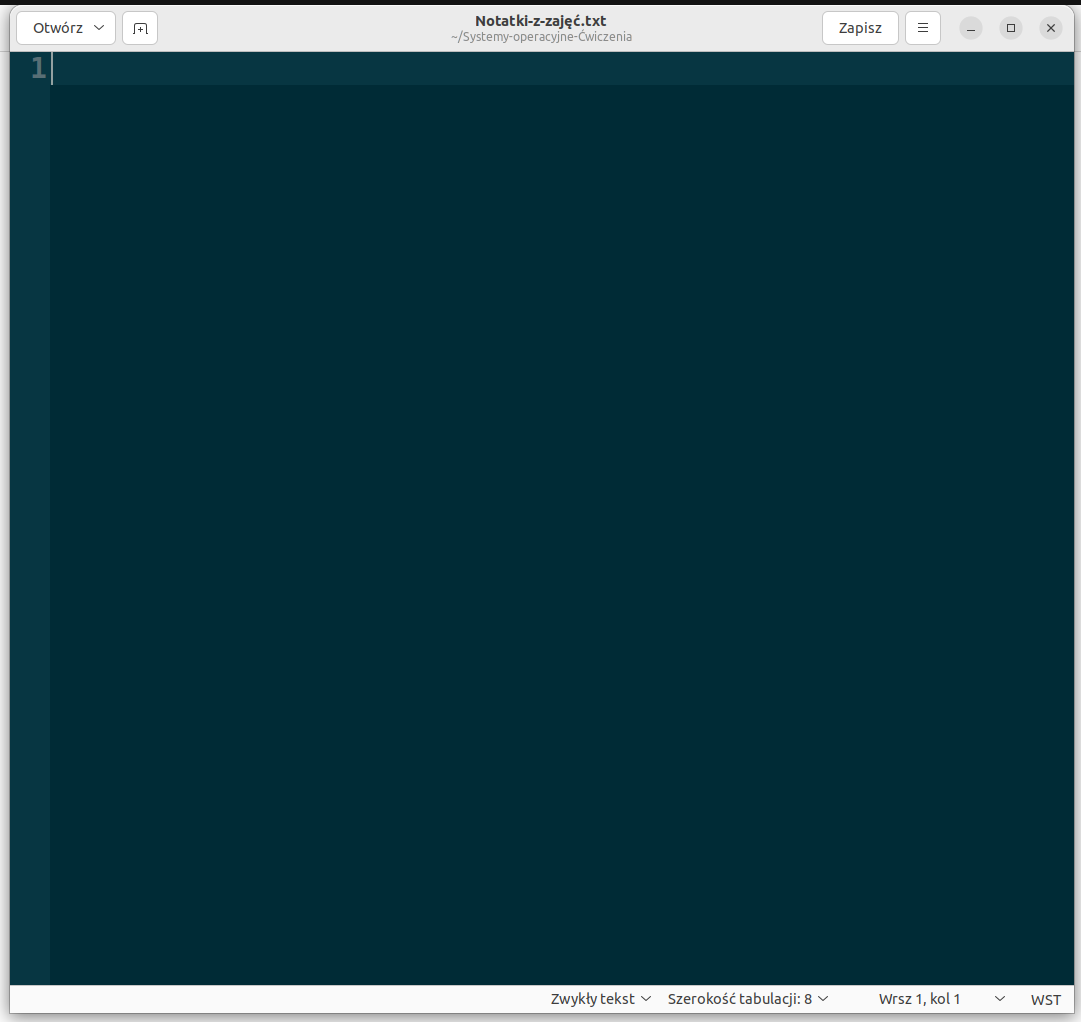
\includegraphics[scale=0.145]
    {./Presentations-pictures/Miscancellous-pictures/gedit-window.png}

    \caption{Otwarte okienko programu gedit.}


    \label{fig:Gedit-window}

  \end{figure}

\end{frame}
% ##################





% ##################
\begin{frame}
  \frametitle{Edytory tekstów}


  Teraz możemy do pliku \texttt{Notatki-z-zajęć.txt} wpisać tekst, choćby
  \textit{Notatki z~przedmiotu „Systemy operacyjne”}. Proszę pamiętać, by
  zapisywać wprowadzone zmiany, służy do tego choćby skrót~\texttt{Ctrl-s}.

  Kilka słów dlaczego wybraliśmy do~edycji plików program gedit. Na~tym
  kursie korzystamy głównie z~niego, gdyż jest on prosty w~obsłudze
  i~w~kilka sekund po jego otwarciu użytkownik może już pisać odpowiedni
  tekst. Zostawiamy jednak Państwu pełną swobodę w~wyborze edytora tekstu.
  Nie jest ważne jakiego programu~się używa, ważne jest, żeby udało~się
  wykonać zadanie jakie przed nami stoi.

  Jeśli chodzi o~edytory dostępne pod systemem GNU/Linux, to w~naszej
  ocenie warto zwrócić uwagę choćby na~dwa owiane już legendą programy
  do edycji tekstu \colorhref{https://www.vim.org/}{vim}
  i~\colorhref{https://www.gnu.org/software/emacs/}{GNU Emacs}.

\end{frame}
% ##################










% ################################################
\section{Czy tylko mi~się wydaje, że~ten system jest dziwny?}
% ################################################


% ######################################
\begin{frame}
  \frametitle{Czy tylko mi~się wydaje, że~ten system jest dziwny?}


  Niejedna z~poznanych przez nas cech systemu operacyjnego, może
  wydawać~się nam dziwna. Czy życie nie mogłoby być prostsze, a~system
  operacyjny bardziej zrozumiały? Odpowiedź na oba pytania brzmi
  „Prawdopodobnie tak”. Dlaczego więc tak nie jest?

  Warto sobie uświadomić, że~niektórzy jeżdżą jeszcze zabytkowymi
  samochodami wyprodukowanymi w~latach $60$-tych XX~wieku. Prawdopodobnie
  gdzieś na świecie działają jakieś komputery wyprodukowane w~tych latach,
  ale większa jest szansa zobaczenia go w~muzeum, niż wykonującego jakąś
  pracę. W~przeciwieństwie do tego, pomysł z~lat $60$-tych mają~się
  świetnie, również w~informatyce. Pracując z~systemami często
  napotykamy~się na jakiś jego fragment, który wymyślono w~owym czasie,
  odbija on więc ówczesny stan wiedzy i~możliwości techniczne. By więc
  zrozumieć pewne osobliwości systemów operacyjnych warto udać~się w~krótką
  podróż w~przeszłość.

\end{frame}
% ######################################





% ######################################
\begin{frame}
  \frametitle{Trochę historii}


  Główne przesłanie tej historii jest następujące. Systemy operacyjne
  których dziś używamy, wyewoluowały do swojej obecnej formy formy
  na przestrzeni dekad, wchłaniając i~łącząc pomysły pochodzące
  z~różnorakich źródeł. Stąd ich dzisiejszy czas może sprawiać wrażenie
  przestarzałego, bałaganiarskiego i~pełnego niekonsekwencji. Jest to prawdą
  w~przypadku w~zasadzie wszystkich popularnych systemów operacyjnych, nie
  tylko omawianego przez nas GNU/Linuxa.

  Zaczynamy w~późnej epoce brązu komputerów, czyli roku~$1965$.
  W~owym roku w~USA, uczelnia M.I.T oraz firmy General Electrics i~Bell
  Labs zaczynają pracę nad systemem operacyjnym
  \colorhref{https://en.wikipedia.org/wiki/Multics}{\textsc{multics}}
  (ang.~\textit{MULTiplexed Information and Computing Service}). Prace
  nas systemem \textsc{multics} okazały~się wyjątkowo skomplikowane i~sam
  projekt odniósł jedynie częściowy sukces. Z~uwagi na trudności
  przy tworzeniu tego systemu Bell Labs wycofały~się z~projektu
  w~roku $1969$.

\end{frame}
% ######################################





% ######################################
\begin{frame}
  \frametitle{Ken Thompson i~jego współpracownicy}


  Jednym z~ludzi, który pracował z~ramienia Bell Labs nad \textsc{multics}em
  jest \colorhref{https://en.wikipedia.org/wiki/Ken\_Thompson}
  {Ken Thompson}. Po wycofaniu~się Bell Labs z~tego projektu, Thompson
  poszukując nowych problemów do rozwiązania, zaczyna pisać programy na
  znajdujący~się w~Bell Labs i~wówczas już rzadko używany komputer
  \colorhref{https://en.wikipedia.org/wiki/PDP-7}{PDP-$7$}.
  W~trackie pracy nad nimi w~pewnym momencie dochodzi do~wniosku,
  że~niewiele mu brakuje do stworzenia systemu operacyjnego. W~ten sposób
  powstaje system operacyjny \textsc{unix}, którego pierwsza wersja
  jest gotowa na jesień $1969$~roku.

  Sama nazwa „\textsc{unix}”,
  jak zgadzają~się wszyscy biorący udział w~jego tworzeniu, jest
  nawiązaniem, i~to dość złośliwym do nazwy „\textsc{multics}”.
  Związane jest to z~powszechną krytyką, że~\textsc{multics} próbował
  osiągnąć zbyt wiele rzeczy na raz i~to nie wyszło mu na zdrowie,
  a~nowy system będzie skupiał~się na robieniu kilku rzeczy dobrze. Stąd
  „multi” zmieniono na „unit” i~powstała nazwa \textsc{unix}, por.
  str.~???.

\end{frame}
% ######################################





% ######################################
\begin{frame}
  \frametitle{Ken Thompson i~jego współpracownicy}


  Do Thompsona w~pracy nad \textsc{unix}em dołącza wielu wybitnych
  informatyków, pracujących wtedy w~Bell Labs, jak ???

  System \textsc{unix} jest pierwszym bezpośrednim przodkiem używanego
  przez nas systemu GNU/Linux, jednak droga od jednego do~drugiego
  jest dość długa i~wyboista.

\end{frame}
% ######################################





% ######################################
\begin{frame}
  \frametitle{Ken Thompson i~jego współpracownicy}



  \begin{figure}

    \centering


    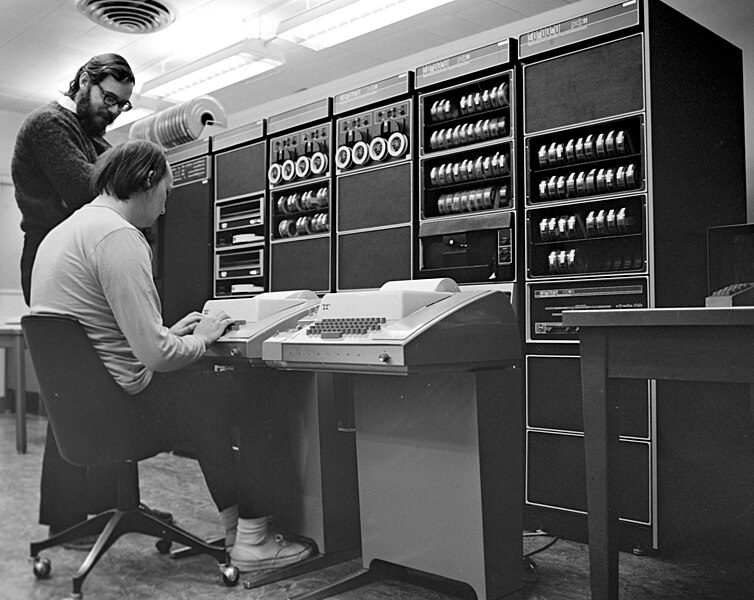
\includegraphics[scale=0.3]
    {./Presentations-pictures/OS-heroes-Pictures/Dennis-Ritchie-Ken-Thompson-around-year-1972.jpg}


    \caption{Ken Thompson (siedzi) i~Dennis Ritchie przy komputerze
      typu PDP-$11$, około roku $1972$-ego.}


    \label{fig:Ritchie-Thompson-around-year-1972}

  \end{figure}

\end{frame}
% ######################################





% ######################################
\begin{frame}
  \frametitle{Ken Thompson i~jego współpracownicy}


  Zdjęcie \eqref{fig:Ritchie-Thompson-around-year-1972} przedstawia Kena
  Thompsona i~Denisa Ritchiego pracujących na komputerze typu
  \colorhref{https://en.wikipedia.org/wiki/PDP-11}{PDP-$11$}, za~pomocą
  dalekopisu
  \colorhref{https://en.wikipedia.org/wiki/Teletype\_Model\_33}
  {Model~$33$ Teletype}. Współtwórca \textsc{unix}a Brian
  W.~Kernighan opatrzył to zdjęcie takim komentarzem.

  \textit{Rysunek 3.1 [u~nas \eqref{fig:Ritchie-Thompson-around-year-1972}]
    przedstawia zrobione na~potrzeby} public relations \textit{w~$1972$
    zdjęcie Kena Thompsona i~Dennisa Ritchiego pracujących nad PDP-$11$
    wyposażona we wczesną wersję Uniksa. Sam komputer najprawdopodobniej
    był specyficznym wariantem PDP-$11$ o~nazwie PDP-$11/20$. Niewielkie,
    okrągłe obiekty znajdujące~się mniej więcej na wysokości głowy, to
    DECtapes~-- napędy z~taśmą magnetyczną, które umożliwiały przechowywanie
    $144\text{K}$ słów $18$-bitowych [$324$ kilobajty pamięci]. Ponieważ
    pozwalały one na odczyt i~zapis pojedynczych bloków, mogły służyć jako
    tymczasowe, wolne, ale niezawodne dyski; taśmy były wymienne, używano
    ich więc też do~archiwizacji danych.}
  Str.~$64$, \parencite{Kernighan-Jak-Unix-tworzyl-historie-Pub-2021}.

\end{frame}
% ######################################





% ######################################
\begin{frame}
  \frametitle{Ken Thompson i~jego współpracownicy}


  \textit{Ken pisze na dalekopisie Model~$33$ Teletype~-- solidnym,
    ale~wolnym i~hałaśliwym urządzeniu, będącym w~istocie sterowaną przez
    komputer elektromechaniczną maszyną do~pisania, która potrafiła pisać
    tylko dużymi literami, w~tempie do~$10$ znaków na sekundę. Model~$33$
    pochodzi z~$1963$ roku, ale wcześniejsze wersje były w~powszechnym
    użyciu już od początku lat~$30$.}

  \textit{Teletype Corporation była częścią AT\&T i~urządzenia Teletypes
    były powszechnie używane w~Bell System i~innych ośrodkach
    do~wysyłania wiadomości; dopiero w~późniejszym czasie zaczęto
    podłączać je do komputerów. To, co zostało wprowadzone na klawiaturze
    Teletype, trafiało do~komputera, a~rezultaty były drukowane (dużymi
    literami) na długiej roli papieru; na~zdjęciu~są widoczne górne
    fragmenty tych rolek. Jak sądzę, jednym z~powodów bardzo krótki
    nazw wielu poleceń Uniksa było to, że~pisanie na Modelu~$33$ wymagało
    niemałej siły, a~drukowanie przebiegało wolno.}
  Str.~$65$, \parencite{Kernighan-Jak-Unix-tworzyl-historie-Pub-2021}.

\end{frame}
% ######################################






% ######################################
\begin{frame}
  \frametitle{Dlaczego?}


  Jak Państwo widzą,

\end{frame}
% ######################################





% ######################################
\begin{frame}
  \frametitle{To tylko część tej historii}


  To co przedstawiliśmy tutaj jest tylko drobnym wycinkiem historii, która
  doprowadziła do powstania używanych przez nas systemów operacyjnych,
  takich jak GNU/Linux.

  Jeśli ktoś chce lepiej poznać tę historię to powinien w~pierwszym rzędzie
  sięgnąć do krótkiej i~bardzo pięknej książki Briana W.~Kernighan
  \textit{Jak Unix tworzył historię}
  \parencite{Kernighan-Jak-Unix-tworzyl-historie-Pub-2021}, która była
  już przez nas wielokrotnie cytowana. Jak sama jej tytuł wskazuje, książka
  ta dotyczy głównie systemu \textsc{unix}, jego powstania i~rozwoju. Jednak
  w~ostatniej części, głównie w~rozdziałach ??? i~??? opisuje drogę, jaka
  wiodła od~\textsc{unix}, do~systemu GNU/Linux. Cała zaś książka jest
  kopalnią informacji na temat, tego kiedy, gdzie i~dlaczego powstały znane
  nam dziś części naszych systemów operacyjnych.

\end{frame}
% ######################################



% % ##################
% \jagiellonianendslide{?????}
% % ##################
















% % ######################################
% \section{Polecenia \textsc{bash}a, ciąg dalszy}
% % ######################################


% % ##################
% \begin{frame}
%   \frametitle{Przesyłanie wielu argumentów do polecenia}


%   Wiele poleceń \textsc{bash}a może przyjąć jako swoje argumenty więcej
%   niż jedną nazwę obiektu, wyjaśnimy to na przykładzie. Materiały
%   dla tego przykładu można znaleźć
%   w~\texttt{Materiały-do-prezentacji/SO-03-A-Polecenia-BASHa-ETC/}.

%   W~katalogu \texttt{SO-03-A-Polecenia-BASHa-ETC/} w~którym~się znajdujemy
%   są m.in. pliki \texttt{Data-01.dat} i~\texttt{Data-02.dat} oraz katalog
%   \texttt{Data-for-analysis/}. Aby przenieść oba pliki z~danymi do
%   wspomnianego katalogu wystarczy jedno polecenie: \\
%   \texttt{\$ mv Data-01.dat Data-02.dat Data-for-analysis/} \\
%   Tak samo możemy przynieść do katalogu trzy lub więcej plików: \\
%   \texttt{\$ mv Data-01.dat Data-02.dat Data-03.dat Data-for-analysis/}

%   Należy dodać, że~katalog do którego przenosimy dwa lub więcej plików,
%   \alert{zawsze} musi być ostatnim argumentem przesłanym do~\texttt{mv}. \\
%   \texttt{\$ mv Data-01.dat Data-for-analysis/ Data-02.dat} \\
%   \texttt{mv: cel 'Data-02.dat' nie jest katalogiem}

% \end{frame}
% % ##################





% % ##################
% \begin{frame}
%   \frametitle{Przesyłanie wielu argumentów do polecenia}


%   \texttt{\$ mv Data-01.dat Data-for-analysis/ Data-02.dat} \\
%   Problem z~powyższym poleceniem polega na tym, że~twórcy polecenia
%   \texttt{mv}, nie potrafili wymyślić, co w~zasadzie miałoby takie jego
%   wywołanie znaczyć. Nie możemy przenieść pliku \texttt{Data-01.dat}
%   i~katalogu \texttt{Data-for-analysis/} do pliku \texttt{Data-02.dat},
%   bo przecież plik nie służy do przechowywania plików lub katalogów.

%   Może więc użytkownik chciał zmienić nazwę jednego z~tych plików?
%   Jeśli tak, to którego i~na co? Czyżby chciał zmienić nazwę pliku
%   \texttt{Data-01.dat} na nazwę katalogu \texttt{Data-for-analysis/}?
%   Rozważania tego typu pokazują, że~decyzja twórców tego polecenia,
%   by~uznać, że~przesłanie do~\texttt{mv} trzech lub więcej argumentów,
%   przy czym ostatni z~nich \alert{nie} jest katalogiem, uznać za błąd
%   użytkownika, była bardzo rozsądna.

%   % Analogicznie, możemy za~pomocą jednego polecenia \texttt{touch} utworzyć
%   % dwa lub więcej plików: \\
%   % \texttt{\$ touch File-01.txt File-02.txt}

%   % W~tym miejscu musimy dodać, że~istnieją znacznie potężniejsze, ale też
%   % bardziej skomplikowane, metody przesyłania nazw wielu obiektów do jednego
%   % polecenia. Ich omówienie odkładamy do momentu, gdy zapoznamy~się już
%   % z~podstawowymi sposobami korzystania z~powłoki.

%   % Zwykle dość łatwo poprawnie zgadnąć, czy dane polecenie może przyjąć
%   % wiele argumentów, czy tylko jedne. Mianowicie, jeśli jest dość oczywiste,
%   % że~dane polecenie można zastosować dla wielu argumentów, to zapewne
%   % działa właśnie tak jak myślimy. Na razie takie podejście powinno nam
%   % wystarczyć.

% \end{frame}
% % ##################





% % ##################
% \begin{frame}
%   \frametitle{Przesyłanie wielu argumentów do polecenia}


%   % \texttt{\$ mv Data-01.dat Data-for-analysis/ Data-02.dat} \\
%   % Problem z~powyższym poleceniem polega na tym, że~twórcy polecenia
%   % \texttt{mv}, nie potrafili wymyślić, co w~zasadzie miałoby takie jego
%   % wywołanie znaczyć. Nie możemy przenieść pliku \texttt{Data-01.dat}
%   % i~katalogu \texttt{Data-for-analysis/} do pliku \texttt{Data-02.dat},
%   % bo przecież plik nie służy do przechowywania plików lub katalogów.

%   % Może więc użytkownik chciał zmienić nazwę jednego z~tych plików?
%   % Jeśli tak, to którego i~na co? Czyżby chciał zmienić nazwę pliku
%   % \texttt{Data-01.dat} na nazwę katalogu \texttt{Data-for-analysis/}?
%   % Rozważania tego typu pokazują, że~decyzja twórców tego polecenia,
%   % by~uznać, że~przesłanie do~\texttt{mv} trzech lub więcej argumentów,
%   % przy czym ostatni z~nich \alert{nie} jest katalogiem, uznać za błąd
%   % użytkownika, była bardzo rozsądna.

%   Analogicznie, możemy za~pomocą jednego polecenia \texttt{touch} utworzyć
%   dwa lub więcej plików: \\
%   \texttt{\$ touch File-01.txt File-02.txt}

%   W~tym miejscu musimy dodać, że~istnieją znacznie potężniejsze, ale też
%   bardziej skomplikowane, metody przesyłania nazw wielu obiektów do jednego
%   polecenia. Ich omówienie odkładamy do momentu, gdy zapoznamy~się już
%   z~podstawowymi sposobami korzystania z~powłoki.

%   Zwykle dość łatwo poprawnie zgadnąć, czy dane polecenie może przyjąć
%   wiele argumentów, czy tylko jedne. Mianowicie, jeśli jest dość oczywiste,
%   że~dane polecenie można zastosować dla wielu argumentów, to zapewne
%   działa właśnie tak jak myślimy. Na razie takie podejście powinno nam
%   wystarczyć.

% \end{frame}
% % ##################





% % ##################
% \begin{frame}
%   \frametitle{Polecenia i~ścieżki do plików oraz katalogów}


%   Załóżmy teraz, że~w~katalogu \texttt{Data-for-analysis/} chcemy utworzyć
%   katalog \texttt{Data-January/}. Żeby to zrobić możemy wejść do tego
%   katalogu i~użyć tam polecenia \texttt{mkdir} tak jak przedstawiono to
%   poniżej. \\
%   \texttt{\$ cd Data-for-analysis/} \\
%   \texttt{\$ mkdir Data-January/}

%   Taki sam rezultat otrzymamy, jeśli poleceniu \texttt{mkdir} prześlemy jako
%   argument ścieżkę katalogu, który chcemy utworzyć. \\
%   \texttt{\$ mkdir Data-for-analysis/Data-January/} \\
%   Zauważmy, że~do polecenia tego przesłaliśmy ścieżkę do~katalogu,
%   który \alert{jeszcze} nie istniał. Jest to zupełnie normalne, wszak
%   polecenie to służy do tworzenia nowych katalogów. To~i~inne polecenia,
%   które służą do tworzenia plików oraz katalogów, w~$99.999\%$ przypadków
%   poprawnie „domyślą~się” co mają utworzyć.

% \end{frame}
% % ##################





% % ##################
% \begin{frame}
%   \frametitle{Polecenia i~ścieżki do plików oraz katalogów}


%   Oczywiście ścieżki przesyłane do~\texttt{mkdir} mogą być dużo dłuższe.
%   Długość ścieżki nie ma naprawdę znaczenia, byleby tylko wskazywała ona
%   na~poprawną lokalizację miejsca, gdzie ma zostać utworzony katalog.

%   Należy jednak zaznaczyć, że~polecenie \texttt{mkdir} zostało napisane tak,
%   że~standardowo można utworzyć tylko ostatni katalog pojawiający~się
%   w~danej ścieżce. Przykładowo, jeśli wpiszemy \\
%   \texttt{\$ mkdir Data-for-analysis/Data-February/Special-data/} \\
%   to zobaczymy komunikat typu \\
%   \texttt{mkdir: nie można utworzyć katalogu
%     „Data-for-analysis/Data-February/Special-data/: Nie ma takiego
%     pliku ani katalogu}

%   Jest tak dlatego, że~wymagałoby to utworzenia najpierw katalogu
%   \texttt{Data-February/}, a~potem utworzenia wewnątrz niego katalogu
%   \texttt{Special-data/}. Ponieważ jednak \texttt{mkdir} stworzono w~taki
%   sposób, że~ma prawo utworzyć tylko ten katalog, który jest na końcu
%   podanej ścieżki, czyli \texttt{Special-data/}, więc polecenie to zgłasza
%   błąd.
%   % Załóżmy teraz, że~w~katalogu \texttt{Data-for-analysis/} chcemy utworzyć
%   % katalog \texttt{Data-January/}. Żeby to zrobić możemy wejść do tego
%   % katalogu i~użyć tam polecenia \texttt{mkdir} tak jak przedstawiono to
%   % poniżej. \\
%   % \texttt{\$ cd Data-for-analysis/} \\
%   % \texttt{\$ mkdir Data-January/}

%   % Taki sam rezultat otrzymamy, jeśli poleceniu \texttt{mkdir} prześlemy jako
%   % argument ścieżkę katalogu, który chcemy utworzyć. \\
%   % \texttt{\$ mkdir Data-for-analysis/Data-January/} \\
%   % Zauważmy, że~do polecenia tego przesłaliśmy ścieżkę do~katalogu,
%   % który \alert{jeszcze} nie istniał. Jest to zupełnie normalne, wszak
%   % polecenie to służy do tworzenia nowych katalogów. To~i~inne polecenia,
%   % które służą do tworzenia plików oraz katalogów, w~$99.999\%$ przypadków
%   % poprawnie „domyślą~się” co mają utworzyć.

% \end{frame}
% % ##################





% % ##################
% \begin{frame}
%   \frametitle{Opcja \texttt{-p} polecenia \texttt{mkdir}}


%   Poprzednio powiedzieliśmy, że~polecenie \\
%   \texttt{\$ mkdir Data-for-analysis/Data-February/Special-data/} \\
%   nie zadziała, bo standardowo \texttt{mkdir} może utworzyć tylko ostatni
%   katalog w~podanej ścieżce. Ale czy jest możliwe włączenie takiego
%   niestandardowego działania?

%   Odpowiedź jest twierdząca. Jeśli poleceniu \texttt{mkdir} dodamy
%   opcję \texttt{-p} to będzie ono mogło utworzyć wszystkie, w~tej
%   chwili jeszcze nieistniejące, katalogi w~podanej ścieżce. Tym samym
%   polecenie \\
%   \texttt{\$ mkdir -p Data-for-analysis/Data-February/Special-data/} \\
%   zadziała poprawnie.

%   Istnieje drugi, zupełnie równoważny zapis, opcji \texttt{-p}, mianowicie
%   \texttt{--parents}. Oznacza to, że~dwa polecenia \\
%   \texttt{\$ mkdir -p Level-01/Level-02/} \\
%   \texttt{\$ mkdir --parents Level-01/Level-02/} \\
%   robią dokładnie to samo.

% \end{frame}
% % ##################





% % ##################
% \begin{frame}
%   \frametitle{Opcja \texttt{-p} polecenia \texttt{mkdir}}


%   Ktoś mógłby sobie zadać pytanie „Czy życie nie jest już wystarczająco
%   skomplikowane, żeby jeszcze nadawać jednej opcji dwie różne nazwy?”
%   Niestety, to kolejna rzecz do której musimy przywyknąć przy pracy
%   w~\textsc{bash}u. Bardzo możliwe, że~gdybyśmy tworzyli obecnie jakiś
%   system operacyjny od~zera, to unikalibyśmy powstania takich sytuacji,
%   jednak gdy chodzi o~systemy istniejące do dekad, takie jak GNU/Linux,
%   musimy zaakceptować je takimi jakimi są.

%   Zwróćmy uwagę na jeszcze jedną rzecz. Opcja \texttt{-p} jest po prostu
%   skrótem od \texttt{--parents}, dlaczego jednak używamy tu słowa
%   oznaczającego „rodziców”? Ogólnie, jeśli mamy katalog \texttt{Level-01/}
%   zawiera katalog \texttt{Level-02/}, to mówimy, że~\texttt{Level-01/}
%   jest \textbf{rodzicem} katalogu \texttt{Level-02/}, a~\texttt{Level-02/}
%   jest \textbf{dzieckiem} katalogu \texttt{Level-01/}.

%   Terminologia ta jest używana do wielu rzeczy w~informatyce, powiem o~niej
%   więcej, gdy będziemy omawiać dokładniej system plików systemu GNU/Linux.

% \end{frame}
% % ##################





% % ##################
% \begin{frame}
%   \frametitle{Jeszcze o~poleceniu \texttt{mkdir}}


%   Dla porządku zaznaczymy, że~pojedyncze polecenie \texttt{mkdir} może bez
%   problemu utworzyć dwa lub więcej katalogów, jeśli tylko podamy ich nazwy
%   (ścieżki) jako dwa osobne argumenty. Przykładowo \\
%   \texttt{\$ mkdir Data-February/ Data-March/} \\
%   utworzy w~katalogu w~którym~się znajdujemy dwa katalogi o~wymienionych
%   wyżej nazwach.

%   Co jednak jeśli katalog \texttt{Data-February/} jeszcze nie istnieje,
%   a~my wprowadzimy następujące polecenie? \\
%   \texttt{\$ mkdir Data-February/ Data-February/Special-data/} \\
%   Mówiąc zupełnie otwarcie, tego typu polecenia każdy musi przetestować
%   na~własną odpowiedzialność. My stoimy na stanowisku, że~najlepiej jest
%   takich rzeczy unikać, bo zysk z~ich stosowania jest niewielki, za~to
%   problemy do jakich mogą prowadzić, potrafią być bardzo duże. Jedna
%   z~mądrości informatyki mądrze mówi: \\
%   \texttt{Better to be clear, than clever.}

% \end{frame}
% % ##################





% % ##################
% \begin{frame}
%   \frametitle{Polecenia i~ścieżki}


%   W~ogólności, należy przyjąć, że~w~każdym poleceniu, którego argumentem
%   może być nazwa pliku lub katalogu, może wystąpić też dowolnie
%   skomplikowana ścieżka do~niego. Zawsze możemy jako argumentu polecenia
%   przesłać ścieżkę bezwzględna, czyli taką, która zaczyna~się od symbolu
%   katalogu root „\texttt{/}”. Jeśli chodzi o~ścieżki względne, to prawie
%   zawsze są one poprawnymi argumentami, acz niekiedy można~się natknąć na
%   pewne wyjątki od~tej reguły.

%   Rozpatrzmy teraz odrobinę inny przykład. Załóżmy teraz, że~w~katalogu
%   gdzie jesteśmy, znajduje~się katalog \texttt{Data-for-analysis/}
%   i~chcemy zobaczyć jego zawartość. Jak poprzednio, żeby to zrobić wystarczy
%   wpisać polecenie \\
%   \texttt{\$ ls Data-for-analysis/} \\
%   \texttt{Data-01.dat} \quad \texttt{Data-02.dat} \\
%   Również tutaj, długość ścieżki nie ma znaczenie, ważne jest jedynie,
%   czy~jest ona poprawna.

% \end{frame}
% % ##################





% % ##################
% \begin{frame}
%   \frametitle{Polecenia i~ścieżki}


%   Przykładowo, zakładając, że~poniższa ścieżka do~katalogu
%   \texttt{Data-for-analysis/} jest poprawna, możemy ten sam rezultat uzyskać
%   pisząc \\
%   \texttt{ls /home/adam/Data-directory/Data-for-analysis/}

%   Niektórym z~Państwa może~się pojawić w~głowie takie pytanie. „Dlaczego
%   teraz przesłaliśmy argument do polecenia \texttt{ls}, choć wcześniej
%   wywoływaliśmy je bez żadnego argumentu?” Nie wchodząc w~szczegóły,
%   w~poprzednich przypadkach polecenie \texttt{ls} samo znajdowało sobie
%   argument, a~był nim bieżący katalog. To powinno być dość proste
%   do~zrozumienia z~kontekstu, dlatego nie będziemy zbyt często
%   zagłębiać~się w~tego typu kwestie.

% \end{frame}
% % ##################





% % ##################
% \begin{frame}
%   \frametitle{Usuwanie katalogów: polecenie \texttt{rmdir}}


%   Dla zupełności wykładu, wspomnimy trochę o~tym jak możemy usunąć
%   niepotrzebny katalog. Do usuwania katalogów należy w~pierwszy rzędzie
%   użyć bardzo bezpiecznego polecenia \texttt{rmdir}: \\
%   \texttt{\$ rmdir Niepotrzebny-katalog/} \\
%   Polecenie to odmówi usunięcia danego katalogu, jeśli nie jest on~pusty,
%   chroni więc nas przed usunięciem katalogu zawierającym ważne dane.

%   Oczywiście, czasem tym czego chcemy jest usunięcie katalogu wraz
%   z~plikami które \alert{zawiera}. To oczywiście też jest do za pomocą
%   polecenia powłoki \textsc{bash}, ale ponieważ to polecenie jest
%   niebezpieczne w~użyciu omówimy je dopiero za~jakiś czas.

% \end{frame}
% % ##################










% % ######################################
% \section{Jeszcze o~poruszaniu~się między katalogami}
% % ######################################


% % ##################
% \begin{frame}
%   \frametitle{Rola systemu operacyjnego}


%   Zacznijmy od~przyjęcia, że~jak poprzednio znajdujemy~się w~katalogu
%   \texttt{SO-03-A-Polecenia-BASHa-ETC/}. Tak jak system Windows,
%   GNU/Linux posiada koncepcję plików ukrytych, czyli takich, które
%   normalnie nie~są widoczne dla użytkownika. Ze~względów historycznych,
%   przyjęto zasadę, że~jeśli nazwa pliku zaczyna~się od symbolu~„\texttt{.}”
%   to plik jest niewidocznych dla użytkownika.

%   By zobaczyć wszystkie pliki, które zawiera dany katalog należy
%   do~polecenia \texttt{ls} przesłać opcję~\texttt{-a}
%   (od ang.~\textit{all}). \\
%   \texttt{\$ ls -a} \\
%   \texttt{.} \quad \texttt{..} \quad \texttt{Data-01.dat} \quad
%   \texttt{Data-02.dat} \quad \directoryName{\texttt{Data-for-analysis}} \\
%   Widzimy, że~w~katalogu tym mamy dwa pliki ukryte, o~dość osobliwych
%   nazwach, jedna kropka i~dwie kropki. Pliki te znajdują~się w~praktycznie
%   każdym katalogu w~systemie GNU/Linux, a~ich nazwy to pewnie zaszłość
%   historyczna z~lat $70$-tych XX wieku, kiedy pamięć była bardzo mała
%   i~każdy symbol~się liczył.

% \end{frame}
% % ##################





% % ##################
% \begin{frame}
%   \frametitle{Pliki „\texttt{.}” i~„\texttt{..}”}


%   Zgodnie z~zasadą, że~w~systemie GNU/Linux wszystko jest plikiem, a~co nie
%   jest plikiem jest procesem, pliki „\texttt{.}” i~„\texttt{..}” służą
%   systemowi operacyjnemu do~pracy z~katalogami. Katalog to wszak tylko inny
%   rodzaj pliku.

%   Zacznijmy od~pliku „\texttt{.}”. Plik ten oznacza po prostu katalog
%   w~którym~się znajdujemy. Co więcej możemy za jego pomocą przejść
%   do~katalogu w~którym jesteśmy (czyli nic nie zrobić), za pomocą
%   polecenia: \\
%   \texttt{\$ cd .} \\
%   Jakkolwiek z~praktycznego punktu widzenia to polecenie jest bezużyteczne,
%   warto wiedzieć, że~istnieje i~działa poprawnie.

% \end{frame}
% % ##################














% % ##################
% \begin{frame}
%   \frametitle{Polecenie \texttt{cd}}




% \end{frame}
% % ##################





% % ##################
% \begin{frame}
%   \frametitle{Polecenie \texttt{cd}}



% \end{frame}
% % ##################





% % ##################
% \begin{frame}
%   \frametitle{Edycja plików z~pomocą programu gedit}




% \end{frame}
% % ##################





% % ##################
% \begin{frame}
%   \frametitle{Okienko gedita}


% \end{frame}
% % ##################





% % ##################
% \begin{frame}
%   \frametitle{Edytory tekstów}



% \end{frame}
% % ##################










% % ######################################
% \section{Dalsze informacje o~pracy z~BASHem}
% % ######################################


% % ##################
% \begin{frame}
%   \frametitle{Pewne subtelności}




% \end{frame}
% % ##################





% % ##################
% \begin{frame}
%   \frametitle{Polecenie \texttt{mkdir}}



% \end{frame}
% % ##################





% % ##################
% \begin{frame}
%   \frametitle{Polecenie \texttt{mv}}



% \end{frame}
% % ##################





% % ##################
% \begin{frame}
%   \frametitle{Polecenie \texttt{mv}}




% \end{frame}
% % ##################





% % ##################
% \begin{frame}
%   \frametitle{Zagrożenia jakie stwarza \texttt{mv}}



% \end{frame}
% % ##################





% % ##################
% \begin{frame}
%   \frametitle{Jak rozsądnie korzystać z~\texttt{mv}?}




% \end{frame}
% % ##################





% % ##################
% \begin{frame}
%   \frametitle{Opcje (flagi)}



% \end{frame}
% % ##################





% % ##################
% \begin{frame}
%   \frametitle{Czemu życie nie może być proste?}




% \end{frame}
% % ##################










% % ######################################
% \section{Autouzupełnianie w~BASHu}
% % ######################################


% % ##################
% \begin{frame}
%   \frametitle{Autouzupełnianie w~BASHu}




% \end{frame}
% % ##################





% % ##################
% \begin{frame}
%   \frametitle{Autouzupełnianie w~BASHu}



% \end{frame}
% % ##################





% % ##################
% \begin{frame}
%   \frametitle{Autouzupełnianie w~BASHu}




% \end{frame}
% % ##################










% % ######################################
% \appendix
% % ######################################





% % ######################################
% \EndingSlide{Dziękuję! Pytania?}
% % ######################################










% % ######################################
% \section{Dlaczego BASH~się tak nazywa}
% % ######################################



% % ##################
% \begin{frame}
%   \frametitle{Dlaczego BASH~się tak nazywa?}




% \end{frame}
% % ##################






% % ##################
% \begin{frame}
%   \frametitle{????}




% \end{frame}
% % ##################






% % ##################
% \endingslide???{}
% % ##################



% % % ##################
% % \jagiellonianendslide{?????}
% % % ##################





% ####################################################################
% ####################################################################
% Bibliography

\printbibliography





% ####################################################################
% End of the document

\end{document}
